\documentclass[aps,prb,reprint,amsmath,amssymb,floatfix]{revtex4-2}
\usepackage{graphicx}
\usepackage{dcolumn}
\usepackage{bm}
\usepackage{booktabs}
\usepackage{multirow}
\usepackage{array}
\usepackage{hyperref}
\usepackage{natbib}
\usepackage{amsmath}

\providecommand{\tightlist}{\setlength{\itemsep}{0pt}\setlength{\parskip}{0pt}}
\providecommand{\pandocbounded}[1]{#1}

\begin{document}

\title{Special Optimal Thermal Cell: Correlator-Designed Supercells for Effective-Harmonic Phonons and Thermodynamics}

\author{Albert Linda}
\email{albert.hzbn@gmail.com}
\affiliation{Department of Materials Science and Engineering, Indian Institute of Technology, Kanpur}

\date{\today}

\begin{abstract}

We introduce the Special Optimal Thermal Cell (SOTC), a deterministic
displacement-design strategy for extracting effective second-order interatomic
force constants (IFCs) from small periodic supercells. Inspired by the
Special Quasirandom Structure construction, SOTC chooses collective atomic
displacements by minimizing the mismatch between selected shell-averaged
displacement correlators of the cell and those of a harmonic trial model. A
self-consistent cycle updates the trial phonons from density-functional-theory
(DFT) forces and ridge-regression IFC fits. For the nine systems studied here
(FCC Al, Ag, Au, and Cu; BCC Mo and W; and rocksalt NaCl, MgO, and PbTe), the
reported self-consistency criterion is reached in 2--5 iterations. The
archived calculations use 1--8 displaced configurations per iteration and an
undisplaced reference, corresponding to 4--36 force evaluations rather than
one force evaluation per iteration.
The resulting effective-harmonic phonons give constant-volume heat capacities
within approximately 5\% of experiment for the ionic compounds at their design
temperatures and within 7\% for all nine materials at 300\,K. At the design
temperatures of the metals, the harmonic heat capacity cannot reproduce
electronic and explicit anharmonic contributions above the Dulong--Petit
limit. The primary SOTC benchmarks assess second-order
effective-harmonic and quasi-harmonic observables; they do not establish
equivalence to methods that sample explicit anharmonic free-energy surfaces.
In a separate 100-snapshot canonical validation for Al, NaCl, and W,
symmetry-constrained FC2+FC3+FC4 models reduce held-out force RMSE by
72--94\% relative to matched central finite-displacement phonopy FC2
baselines. This validates the higher-order fitting and export implementation,
not a few-configuration SOTC sampling advantage.  For NaCl, QE DFPT Born
charges and the electronic dielectric tensor produce a 2.895\,THz LO--TO
splitting when applied to the matched finite-displacement phonons.
The implementation is available as an open-source Python package interfaced
to Quantum ESPRESSO.

\end{abstract}

\maketitle

\section{Introduction}\label{introduction}

High-temperature phonon properties (renormalized dispersions, soft-mode
instabilities, thermal expansion, heat capacity) encode the anharmonic
response of a crystal to atomic vibrations with amplitudes reaching
several percent of the lattice constant. Accurate first-principles
descriptions of these properties are essential for predicting phase
stability \cite{ref1}, thermal conductivity \cite{ref2},
electron--phonon coupling \cite{ref3}, and thermodynamic databases for
materials design \cite{ref4}.

Finite-temperature lattice dynamics can be formulated at several distinct
levels. The temperature-dependent effective potential framework fits effective
second- and higher-order IFCs to finite-temperature force data
\cite{ref5,ref6,ref10,ref52}. Variational self-consistent harmonic methods
optimize a trial distribution and its free energy \cite{ref7,ref8,ref50},
while mode-coupling theory provides a separate non-perturbative description of
anharmonic lattice dynamics \cite{ref51}. Ab initio molecular dynamics samples
classical nuclear trajectories on the chosen electronic potential-energy
surface \cite{ref9}. These approaches do not target identical observables or
approximations; meaningful cost or accuracy comparisons therefore require
matched cells, electronic settings, temperatures, and physical outputs.

In a parallel development, Zunger and coworkers \cite{ref12}
demonstrated that a random substitutional alloy can be mimicked
statistically by a single small supercell, the Special Quasirandom
Structure (SQS), whose chemical correlation functions match those of the
ideal random alloy up to a spatial cutoff. The key observation is that
structure encodes information: the correct spatial correlations are
imposed by construction rather than recovered by averaging over an
ensemble.

We apply the special-structure idea to displacement design. A harmonic trial
model defines displacement--displacement correlations
\(C_{ab}^{\alpha\beta}(\mathbf R,T)\). SOTC searches a fixed periodic
supercell for a collective displacement pattern whose selected shell-averaged
correlators approximate these targets up to the IFC cutoff. DFT forces on the
designed configuration are then used in a symmetry-constrained ridge fit of
second-order IFCs, and the fitted phonons update the target correlators. The
small iteration counts reported below are empirical observations for the
present benchmarks, not a proof that a single configuration identifies an
arbitrary IFC tensor.

SOTC is thus a deterministic configuration-design and effective-FC2 fitting
procedure. It does not minimize an anharmonic variational free energy or
generate a time trajectory. Its proposed distinction is the explicit
optimization of prescribed spatial correlator moments before the force
calculation, rather than a general replacement for ensemble or trajectory
methods.

This paper is organized as follows. Section II presents the theoretical
framework: thermal displacement correlators, the SOTC objective
function, IFC extraction by ridge regression, the self-consistency loop,
and the quasi-harmonic extension for continuous thermodynamic
properties. Section III describes computational details. Section IV
reports benchmarks for all nine materials, including thermal expansion
for aluminum (Sec. IV.F). Section V discusses the method's range of
validity, limitations, computational cost, and comparison with the
phonopy quasi-harmonic approximation (QHA). Section VI concludes.

\section{Theory}\label{theory}

\subsection{Thermal Displacement
Correlators}\label{thermal-displacement-correlators}

Consider a crystal with \(n_b\) basis atoms and \(N_c=N_1N_2N_3\)
primitive cells, so that the supercell contains \(n_bN_c\) atoms. Let
\(u_a^\alpha(\mathbf R)\) be the displacement of basis atom \(a\) in cell
\(\mathbf R\). With the Fourier convention defined in Appendix~A, the
equal-time canonical correlator of a harmonic lattice is \cite{ref13}:

{\footnotesize
\begin{align}
C_{ab}^{\alpha\beta}(\mathbf{R},T)
  &= \langle u_a^\alpha(\mathbf{0})\, u_b^\beta(\mathbf{R})\rangle_T \nonumber \\
  &= \frac{\hbar}{2N_c\sqrt{M_a M_b}} \sum_{\mathbf{q},s}
     \frac{e_a^{\alpha*}(\mathbf{q}s)\,e_b^{\beta}(\mathbf{q}s)}{\omega_{\mathbf{q}s}}
     \coth\!\left(\frac{\hbar\omega_{\mathbf{q}s}}{2k_BT}\right)
     e^{-i\mathbf{q}\cdot\mathbf{R}} .
\end{align}
}

Here \(\mathbf q\) runs over the \(N_c\) wave vectors commensurate with the
Born--von K\'arm\'an cell, \(s\) labels a phonon branch, and the polarization
vectors obey the normalization stated in Appendix~A. The remaining symbols
have their usual meanings. Equation~(1) is standard harmonic-lattice theory;
a derivation and the phase convention are given in Appendix~A.

The \(\coth\) factor encodes the full quantum Bose--Einstein statistics,
smoothly interpolating between the zero-point limit (\(T\to 0\):
\(\coth\to 1\)) and the classical equipartition limit
(\(k_BT\gg\hbar\omega\): \(\coth\to 2k_BT/\hbar\omega\)).

To reduce the tensor correlator to the scalar target used in the present
implementation, let \(\mathcal S_R^{ab}\) denote the set of lattice vectors
belonging to the crystallographic shell of radius \(R\) for basis pair
\((a,b)\), with multiplicity \(N_R^{ab}\). The shell and Cartesian trace
average is defined by
\begin{equation}
\bar C_2^{ab}(R,T)=\frac{1}{3N_R^{ab}}
\sum_{\mathbf R'\in\mathcal S_R^{ab}}\sum_{\alpha}
C_{ab}^{\alpha\alpha}(\mathbf R',T).
\end{equation}
Thus \(R\) labels a discrete neighbor shell; it is not a continuum spherical
average. Numerically equivalent distances are grouped using the distance
tolerance reported with the calculation inputs. Species/basis-pair channels
are retained separately. This scalar reduction discards anisotropic and
off-diagonal correlation information, a limitation discussed in Sec.~V.D.

For a monatomic cubic crystal, the on-site value is the one-component
isotropic displacement parameter
\(U_{\rm iso}=\frac13\langle|\mathbf u|^2\rangle\):
\begin{equation}
U_{\rm iso}(T)=\bar C_2(0,T)=
\frac{\hbar}{6N_cM}\sum_{\mathbf q,s}
\frac{1}{\omega_{\mathbf q s}}
\coth\!\left(\frac{\hbar\omega_{\mathbf q s}}{2k_BT}\right).
\end{equation}
Equation~(3) follows from the trace of Eq.~(1) and the polarization-vector
completeness relation. The total three-dimensional MSD is
\(3U_{\rm iso}\), while crystallographic Debye--Waller factors use
\(B=8\pi^2U_{\rm iso}\). For compounds, species-resolved displacements are
evaluated from the full eigenvector-weighted mode sum rather than a
species-averaged mass and the total DOS. The displacement norm used to design
a SOTC configuration is documented separately from this one-component
quantity to avoid a factor-of-three ambiguity.

\subsection{The SOTC Objective
Function}\label{the-sotc-objective-function}

Let \(\Omega\) be a candidate supercell of \(n\) atoms (with
\(n \ll N\)) and let \(\{\mathbf{u}_i\}\) be a set of atomic
displacements assigned to those atoms.
The \textbf{SOTC objective function} measures the mismatch between the
selected correlators of a finite displacement vector and the harmonic trial
targets:

\begin{equation}
\mathcal{Q}(\mathbf{u}) = \sum_{a,b}\sum_{R<r_\text{cut}} w_{ab}(R)
\left[\bar{C}_{2,ab}^\text{cell}(R;\mathbf u)
- \bar{C}_{2,ab}(R,T)\right]^2 .
\end{equation}

Here \(\bar C_{2,ab}^{\rm cell}\) is formed with the same shell, trace, and
species averaging as Eq.~(2), and \(r_{\rm cut}\) is the real-space IFC
cutoff. Equation~(4) is introduced in this work; its gradient is given in
Appendix~C. A positive distance weight may be chosen, for example
\begin{equation}
w_{ab}(R;\xi_w)=\exp(-R/\xi_w),
\end{equation}
where \(\xi_w\) is a numerical weighting length whose adequacy must be tested
by cutoff and dispersion convergence. We do not identify \(\xi_w\) with a
universal phonon mean free path: a finite dynamical phonon lifetime does not,
by itself, prove exponential decay of an equal-time displacement correlator.
No lifetime-based exponential decay or universal
\(T^{-1}\)/\(T^{-3}\) scaling law is assumed in this formulation.

Minimization of \(\mathcal{Q}\) over the displacement field
\(\{\mathbf{u}_i\}\) subject to \(|\mathbf{u}_i| \leq u_\text{rms}(T)\)
is performed by gradient descent with random restarts. The initial guess
is the harmonic displacement pattern obtained by sampling each phonon
mode with amplitude
\(A_{\mathbf{q}s}^{(0)} = \sqrt{\hbar\coth(\hbar\omega_{\mathbf{q}s}/2k_BT)/2\omega_{\mathbf{q}s}}\).
The optimization adjusts mode amplitudes and phase relations to minimize
the correlator mismatch while keeping displacements physically bounded.

\subsection{IFC Extraction by Ridge
Regression}\label{ifc-extraction-by-ridge-regression}

Let \(F_i^\alpha(\mathbf u)\) and \(F_i^\alpha(\mathbf0)\) be forces on the
displaced and reference structures at the same cell. The response force
\(\Delta F_i^\alpha=F_i^\alpha(\mathbf u)-F_i^\alpha(\mathbf0)\) removes any
residual reference force. To harmonic order, the collective-displacement
relation with translational invariance written explicitly is

\begin{equation}
\Delta F_i^\alpha = -\sum_{j,\beta}
\Phi_{ij}^{\alpha\beta}\,(u_j^\beta-u_i^\beta)
+\mathcal O(u^2).
\end{equation}

This constitutes an underdetermined system when the number of IFC
parameters \(N_\text{IFC}\) exceeds \(3n\) (the dimension of the force
vector). We use Tikhonov (ridge) regression to stabilize the inversion:

\begin{equation}
\hat{\boldsymbol{\Phi}} = -\left(\mathbf{G}^T\mathbf{G} + \lambda\mathbf{I}\right)^{-1} \mathbf{G}^T \Delta\mathbf{F}.
\end{equation}

The geometry matrix \(\mathbf G\) contains the relative displacements in
Eq.~(6), \(\Delta\mathbf F\) stacks the response forces, and \(\lambda\) is the
ridge parameter. Equation~(7) is standard Tikhonov regularization applied to
the symmetry-reduced force model; the constrained construction is detailed in
Appendix~D. The acoustic sum rule is imposed as a hard linear constraint, and
an optional central-force projection further reduces the parameter space.
These constraints, the finite cutoff, and ridge regularization are physical and
statistical priors, and their influence must be distinguished from information
provided by the DFT forces.

For one \(n\)-atom configuration, \(\mathbf G\) has \(3n\) rows and hence
algebraic rank no larger than \(3n\). Full identification requires the rank to
be compared with the number of independent IFC parameters after all symmetry
and sum-rule reductions. Ridge regularization stabilizes a rank-deficient fit
but does not create missing information. The validation therefore reports parameter counts, singular-value tolerance, rank, and condition number
for each actual matrix rather than asserting coverage from the iteration count
alone.

\subsection{Phonon Reconstruction}\label{phonon-reconstruction}

From the extracted IFCs \(\hat{\Phi}_{ij}^{\alpha\beta}(\mathbf{R})\),
the dynamical matrix is constructed as:

\begin{equation}
D_{ij}^{\alpha\beta}(\mathbf{q}) = \frac{1}{\sqrt{M_i M_j}} \sum_{\mathbf{R}} \hat{\Phi}_{ij}^{\alpha\beta}(\mathbf{R})\, e^{i\mathbf{q}\cdot\mathbf{R}}
\end{equation}

Equation~(8) is the standard Fourier construction of the harmonic dynamical
matrix from real-space IFCs \cite{ref13}; the retained real-space cutoff and
non-analytic polar correction determine its domain of validity.

Phonon dispersion: the \(3n_b\) branches \(\omega_{\mathbf{q}s}\) follow
from eigenvalues of \(D(\mathbf{q})\), evaluated on a dense
Monkhorst--Pack grid. The phonon density of states (DOS) is obtained by
linear tetrahedron integration with Gaussian broadening \(\sigma = 0.1\)
THz.

Thermodynamic properties follow directly from the phonon DOS
\(g(\omega)\):

\begin{equation}
C_V(T) = k_B \int_0^{\omega_\text{max}} g(\omega) \left(\frac{\hbar\omega}{2k_BT}\right)^2 \sinh^{-2}\!\left(\frac{\hbar\omega}{2k_BT}\right) d\omega
\end{equation}

\begin{equation}
F_\text{vib}(T) = k_B T \int_0^{\omega_\text{max}} g(\omega) \ln\!\left[2\sinh\!\left(\frac{\hbar\omega}{2k_BT}\right)\right] d\omega
\end{equation}

\begin{equation}
\text{ZPE} = \frac{\hbar}{2}\int_0^{\omega_\text{max}} g(\omega)\,\omega\, d\omega
\end{equation}

\begin{equation}
\begin{aligned}
U_{\rm iso}(T)
 &= \frac{\hbar}{6M}\int_0^{\omega_{\rm max}}
 \frac{g(\omega)}{\omega}
 \coth\!\left(\frac{\hbar\omega}{2k_BT}\right)d\omega,\\
\int_0^{\omega_{\rm max}}g(\omega)d\omega&=3 .
\end{aligned}
\end{equation}

Equation~(12) is the monatomic one-component displacement obtained from
Eq.~(3) when the total DOS is normalized to three modes per atom. For a
compound, species-resolved eigenvector weights and masses are required; a
species-averaged mass multiplying the total DOS is not used. The harmonic
thermodynamic identities in Eqs.~(9)--(12) are standard consequences of the
independent-phonon partition function \cite{ref13}.
The spectral Debye temperature is the second-moment Debye temperature

\(T_D^\text{spec} = (\hbar/k_B)\sqrt{5\langle\omega^2\rangle_g/3}\),
where
\(\langle\omega^2\rangle_g = \int g(\omega)\,\omega^2\,d\omega/\int g(\omega)\,d\omega\)
is the mean-square phonon frequency over the DOS; this uses the Debye
relation \(\langle\omega^2\rangle = 3\omega_D^2/5\). The caloric Debye
temperature \(T_D^\text{cal}(T)\) is defined by inversion of the Debye
model for \(C_V(T)\).

\subsection{Self-Consistent Loop}\label{self-consistent-loop}

The SOTC method is closed into a self-consistency cycle:

\begin{enumerate}
\def\labelenumi{\arabic{enumi}.}
\tightlist
\item
  \textbf{Initialize}: start from a Debye or Einstein trial phonon model
  \(\omega^{(0)}(\mathbf{q})\).
\item
  \textbf{Compute target correlators}: \(\bar{C}_2(R,T)\) from Eqs.
  (1)--(2) using current phonon model.
\item
  \textbf{Design configurations}: with the supercell fixed,
  minimize \(\mathcal Q(\mathbf u)\) [Eq.~(4)] to generate
  \(N_{\rm ens}\) displacement configurations.
\item
  \textbf{DFT forces}: evaluate the undisplaced reference
  and all \(N_{\rm ens}\) displaced configurations.
\item
  \textbf{Extract IFCs}: ridge regression from Eq. (6).
\item
  \textbf{Update phonon model}: diagonalize \(D(\mathbf{q})\) from new
  IFCs.
\item
  \textbf{Check convergence}: the archived benchmarks use
  \(\|\Delta\bar C_2\|_2<3\times10^{-3}\)~Å\(^2\), together with the
  material-specific minimum iteration counts reported in the calculation
  inputs. If not converged, return to step 2.
\end{enumerate}

The Debye or Einstein model supplies only the first target in the intended
self-consistent workflow; subsequent targets depend on the fitted
material-specific IFCs. Nevertheless, the finite-data priors and numerical
safeguards can retain initialization dependence. Validation requires comparison of Debye, Einstein, perturbed, and deliberately poor initial
models rather than assuming a unique fixed point.

Each iteration evaluates \(N_{\rm ens}\) displaced configurations and an
undisplaced reference configuration. In the current implementation the
reference is recomputed once per iteration; hence the force-call count is
\(N_{\rm iter}(N_{\rm ens}+1)\), not \(N_{\rm iter}\). The archived benchmarks
reach their stopping criterion in 2--5 iterations with
\(N_{\rm ens}=1\)--8, as detailed in Table~I. Iteration count is therefore not
used as a proxy for DFT cost.

\subsection{Quasi-Harmonic Approximation and Continuous High-Temperature
Properties}\label{quasi-harmonic-approximation-and-continuous-high-temperature-properties}

The self-consistent SOTC loop delivers converged IFCs
\(\Phi_{ij}^{*\alpha\beta}(T)\) at a single design temperature \(T\). To
obtain continuous thermodynamic properties, specifically the thermal
expansion coefficient \(\alpha(T)\), isobaric heat capacity \(C_P(T)\),
and bulk modulus \(B(T)\), across a temperature range without repeating
the SOTC loop at each \(T\), we couple SOTC phonons to the QHA.

\textbf{SOTC-QHA setup.} A converged QHA calculation requires a set of
\(N_V\) volumes spanning the thermally sampled range. Static reference-lattice
energies \(E_0(V)\) and phonons are computed directly at every volume; energies
of thermally displaced configurations are not substituted for \(E_0\), and
IFCs at an uncalculated volume are not inferred by linear extrapolation. At
least five volumes are used for a third-order Birch--Murnaghan fit, with
convergence checked against the number and range of volumes. The zero-pressure
Helmholtz free energy is
\begin{equation}
F(T,V)=E_0(V)+F_{\rm vib}(T,V),
\end{equation}
where the harmonic vibrational contribution is
\begin{equation}
F_{\rm vib}(T,V)=k_BT\sum_{\mathbf q,s}
\ln\!\left[2\sinh\!\left(\frac{\hbar\omega_{\mathbf q s}(V)}
{2k_BT}\right)\right].
\end{equation}
At external pressure \(p\), the equilibrium volume minimizes
\(F(T,V)+pV\):
\begin{equation}
\left.\frac{\partial [F(T,V)+pV]}{\partial V}\right|_{V^*(T,p)}=0 .
\end{equation}
Thus \(F\), rather than \(G\), is minimized at \(p=0\). Equations
(13)--(15) are the standard quasi-harmonic construction \cite{ref44,ref45};
they do not imply an anharmonic variational upper bound.

For a cubic crystal, define the volumetric and linear expansion coefficients
separately. The thermodynamic identities are
\begin{equation}
\alpha_V=\frac{1}{V^*}\frac{dV^*}{dT},\qquad
\alpha_L=\frac{\alpha_V}{3},\qquad
B_T=V^*\left.\frac{\partial^2F}{\partial V^2}\right|_{V^*}.
\end{equation}
The corresponding heat-capacity relation is
\begin{equation}
C_P-C_V=TV^*B_T\alpha_V^2
       =9TV^*B_T\alpha_L^2 .
\end{equation}
The positive curvature sign, the distinction between \(\alpha_V\) and
\(\alpha_L\), and the factor of nine in the linear-coefficient form are
essential. All numerical QHA results must be regenerated with these conventions
and with a converged volume grid before an accuracy or cost comparison is made.

\textbf{Grüneisen shortcut.} When volume-changing DFT runs are not
desired, a faster estimate uses the mode Grüneisen parameters:

\begin{equation}
\gamma_{\mathbf{q}s} = -\frac{V}{\omega_{\mathbf{q}s}}\frac{\partial\omega_{\mathbf{q}s}}{\partial V}\bigg|_{V_0} \approx -\frac{V_0}{\omega_{\mathbf{q}s}}\frac{\omega_{\mathbf{q}s}(V_+)-\omega_{\mathbf{q}s}(V_-)}{V_+-V_-}
\end{equation}

The heat-capacity-weighted average
\(\gamma_\text{eff}(T) = \sum_{\mathbf{q}s}c_{\mathbf{q}s}(T)\gamma_{\mathbf{q}s}/\sum_{\mathbf{q}s}c_{\mathbf{q}s}(T)\)
gives:

\begin{equation}
\alpha_L(T) \approx
\frac{\gamma_\text{eff}(T)\,C_V(T)}{3B_0V_0},\qquad
\alpha_V(T)=3\alpha_L(T).
\end{equation}

Here \(B_0=V_0(\partial^2E_0/\partial V^2)_{V_0}\) is the positive static
bulk modulus. Equation~(19) is the standard cubic Grüneisen relation
\cite{ref44}; it requires volume derivatives of the phonons and is a diagnostic
approximation, not an independent validation of QHA. Software-specific class
names and keyword choices are moved to the reproducibility material.

\section{Computational Details}\label{computational-details}

\subsection{DFT Calculations}\label{dft-calculations}

All force calculations used Quantum ESPRESSO 7.5 \cite{ref46}, PBE
\cite{ref17}, and pseudopotentials from the SSSP efficiency library
\cite{ref47}. The selected potentials were ONCV for Ag, Au, and Mo; PAW for
Al, Cu, Mg, O, and Pb; and ultrasoft for Na, Cl, Te, and W. Wave-function
cutoffs (Ry) were Al 40, Ag 50, Au 45, Cu 45, Mo 40, W 30, NaCl 60,
MgO 80, and PbTe 44. Charge-density cutoffs were four times the
wave-function cutoff for ONCV and eight times it for PAW/ultrasoft
potentials. FCC and BCC supercells used a Gamma-centered
\(2\times2\times2\) k mesh; rocksalt supercells used Gamma only. Metals used
Marzari--Vanderbilt cold smearing \cite{ref18} of 0.02\,Ry, while the
insulators used fixed occupations. Literal pseudopotential filenames, QE
keywords, and software class/flag names are collected in Appendix~K rather
than the theory section.

Experimental lattice constants and ideal high-symmetry fractional coordinates
were used for the archived benchmarks. An undisplaced single-point calculation
at the same cell defines the reference force and stress. IFC fits use
\(\Delta\mathbf F=\mathbf F(\mathbf u)-\mathbf F(\mathbf0)\), as in Eq.~(6),
rather than assuming \(\mathbf F(\mathbf0)=0\). The calculation archive should report
maximum/RMS reference forces, induced-force scales, residual stresses, and
comparisons with representative PBE-relaxed cells.

\subsection{SOTC Supercell Setup}\label{sotc-supercell-setup}

The supercell geometry (Hermite Normal Form matrix \(\mathbf{H}\)) is
selected once before the self-consistency loop by enumerating all HNF
candidates whose number of primitive cells \(n\) satisfies
\(\max(2,\,n_\text{sc}-2) \le n \le n_\text{sc}\), where
\(n_\text{sc}\) is the user-specified target. Candidates are ranked by a
two-criterion score: nearest-neighbor shell completeness first, then
supercell lattice condition number (a measure of cell cubicity); the best candidate at or below the
target size is adopted. This upper bound ensures the supercell never
exceeds the intended size.

FCC metals (Al, Ag, Au, Cu) used a \(2\times2\times2\) conventional-cell
supercell (4 atoms/cell \(\times\) 8 = 32 atoms); BCC metals (Mo, W)
used a 64-atom supercell (2 atoms/cell \(\times\) 32 conventional cells)
and rocksalt compounds (NaCl, MgO, PbTe) used a \(2\times2\times2\)
conventional-cell supercell (8 atoms/cell \(\times\) 8 = 64 atoms).

The experimental lattice parameters are provided in the archived inputs; Table~I
now reports force-call accounting. The IFC cutoffs are listed in Table~I, and
the ridge parameter was \(10^{-3}\) in the code's reported units. A
central-force bond projection was enabled for all archived benchmarks. Because
this is a strong physical prior rather than a software detail, sensitivity tests should compare it with the less constrained tensor fit.

The archived benchmark workflow used one SOTC displacement configuration per
self-consistency iteration (\(N_{\rm ens}=1\)). This fact does not guarantee
full IFC coverage. For every benchmark, the data release should report
the dimensions and numerical rank of the symmetry-reduced design matrix, its
singular-value threshold and condition number, and the independent parameter
count. The ensemble mode (\(N_{\rm ens}>1\)) provides additional force rows
when an overdetermined fit is required.

\subsection{Phonon Post-Processing}\label{phonon-post-processing}

Phonon DOS calculations used a \(30\times30\times30\) Monkhorst--Pack mesh
(27,000 q points), while band dispersions were interpolated from the real-space
IFCs along the paths stored with the released band data:
\(\Gamma\)-X-W-K-\(\Gamma\)-L for FCC and rocksalt and
\(\Gamma\)-H-N-\(\Gamma\)-P-H for BCC. Thermal properties were computed on an
\(8\times8\times8\)

grid (512 q-points) for \(C_V(T)\), \(F_\text{vib}(T)\), and
\(S_\text{vib}(T)\). Gaussian broadening \(\sigma = 0.1\) THz was
applied to the phonon DOS. Convergence of \(C_V\) with q-mesh was
verified by comparing \(8\times8\times8\) and \(16\times16\times16\)
grids for Al and MgO; the difference is \(< 0.05\) J/(mol·K) in both
cases, confirming that the \(8\times8\times8\) grid is fully converged.

\subsection{Experimental Reference
Data}\label{experimental-reference-data}

Experimental Debye temperatures and heat capacities were taken from the
NIST-JANAF tables \cite{ref20} and Kittel \cite{ref21}. References for
individual systems: Al \cite{ref22,ref23}, Ag \cite{ref23}, Au
\cite{ref24}, Cu \cite{ref25}, Mo \cite{ref26,ref27}, W \cite{ref27},
NaCl \cite{ref28}, MgO \cite{ref29,ref30}, PbTe \cite{ref31,ref32}. For
comparison of phonon dispersions, we use neutron scattering data from:
Cu (Ref. \cite{ref33}), Al (Ref. \cite{ref34}), NaCl (Ref.
\cite{ref35}).

\subsection{SOTC-QHA Setup for
Aluminum}\label{sotc-qha-setup-for-aluminum}

The available Al dataset contains only \(V_0\) and \(V_-\), an
extrapolated expanded-volume IFC matrix, and energies from displaced cells. It
is insufficient for a converged equation of state. A quantitative QHA study
requires direct static reference-lattice energies and direct FC2 phonon
calculations at at least five volumes, followed by volume-grid, EOS, and
temperature-derivative convergence tests as specified in Sec.~II.F. No
numerical Al expansion coefficient or QHA cost/accuracy comparison is therefore
reported.

\section{Results}\label{results}

\subsection{Self-Consistency
Convergence}\label{self-consistency-convergence}

A multi-method Debye-temperature comparison is not shown because the available
external-method series lack calculation-level provenance and matched settings.
The SOTC FC2 and experimental values remain tabulated, but no external-method
accuracy claim is based on those unmatched data.

The archived runs stop after 2--5 self-consistency iterations under the
material-specific minimum-iteration rule and the correlator threshold stated in
Sec.~II.E. This is convergence of the chosen scalar stopping metric, not a
demonstration that the full phonon dispersion is converged. Direct
configuration-count and dispersion-error convergence against a matched
reference is required for that stronger claim.

\begin{table*}[htbp]

\caption{Archived SOTC iteration and force-call accounting.
\(N_{\rm iter}\) is the number of self-consistency iterations,
\(N_{\rm ens}\) the displaced configurations evaluated per iteration,
\(N_{\rm disp}=N_{\rm iter}N_{\rm ens}\), and
\(N_{\rm force}=N_{\rm iter}(N_{\rm ens}+1)\) includes the undisplaced
reference recomputed by the current runner. These counts do not establish IFC
or dispersion convergence.}
\begin{ruledtabular}
\begin{tabular}{lrrrrrrrr}
Material & \(T_{\rm des}\) (K) & \(N_{\rm atoms}\) & \(r_{\rm cut}\) (Å) &
\(N_{\rm iter}\) & \(N_{\rm ens}\) & \(N_{\rm disp}\) &
\(N_{\rm ref}\) & \(N_{\rm force}\) \\
\hline
Al   & 300  & 32 & 4.5 & 2 & 5 & 10 & 2 & 12 \\
Ag   & 1000 & 32 & 4.5 & 4 & 5 & 20 & 4 & 24 \\
Au   & 1200 & 32 & 4.5 & 2 & 1 &  2 & 2 &  4 \\
Cu   & 1200 & 32 & 4.5 & 4 & 8 & 32 & 4 & 36 \\
Mo   & 1500 & 64 & 5.0 & 2 & 1 &  2 & 2 &  4 \\
W    & 1500 & 64 & 5.0 & 4 & 3 & 12 & 4 & 16 \\
NaCl & 700  & 64 & 4.3 & 5 & 3 & 15 & 5 & 20 \\
MgO  & 1500 & 64 & 3.2 & 4 & 3 & 12 & 4 & 16 \\
PbTe & 700  & 64 & 5.0 & 4 & 5 & 20 & 4 & 24 \\
\end{tabular}
\end{ruledtabular}
\label{tab:1}

\end{table*}

Table~I shows that the present runs themselves use ensembles and require
2--32 displaced calculations, or 4--36 force calculations when the repeated
reference evaluations are counted. No external-method cost-reduction factor
is inferred from these numbers
because no comparison dataset was generated with a matched cell,
electronic-structure setup, sampling protocol, IFC rank, and dispersion
accuracy target.

\subsection{Phonon Dispersions and
DOS}\label{phonon-dispersions-and-dos}

Figure~2 displays the SOTC effective-FC2 dispersions and DOS. The curves expose
branch topology and instabilities but do not include explicit FC3 or FC4
self-energies. They are presented descriptively because the cited neutron data
and a matched converged DFT reference are not overlaid; no branch-resolved
accuracy or superiority claim is inferred.

\begin{figure*}[htbp]
\centering
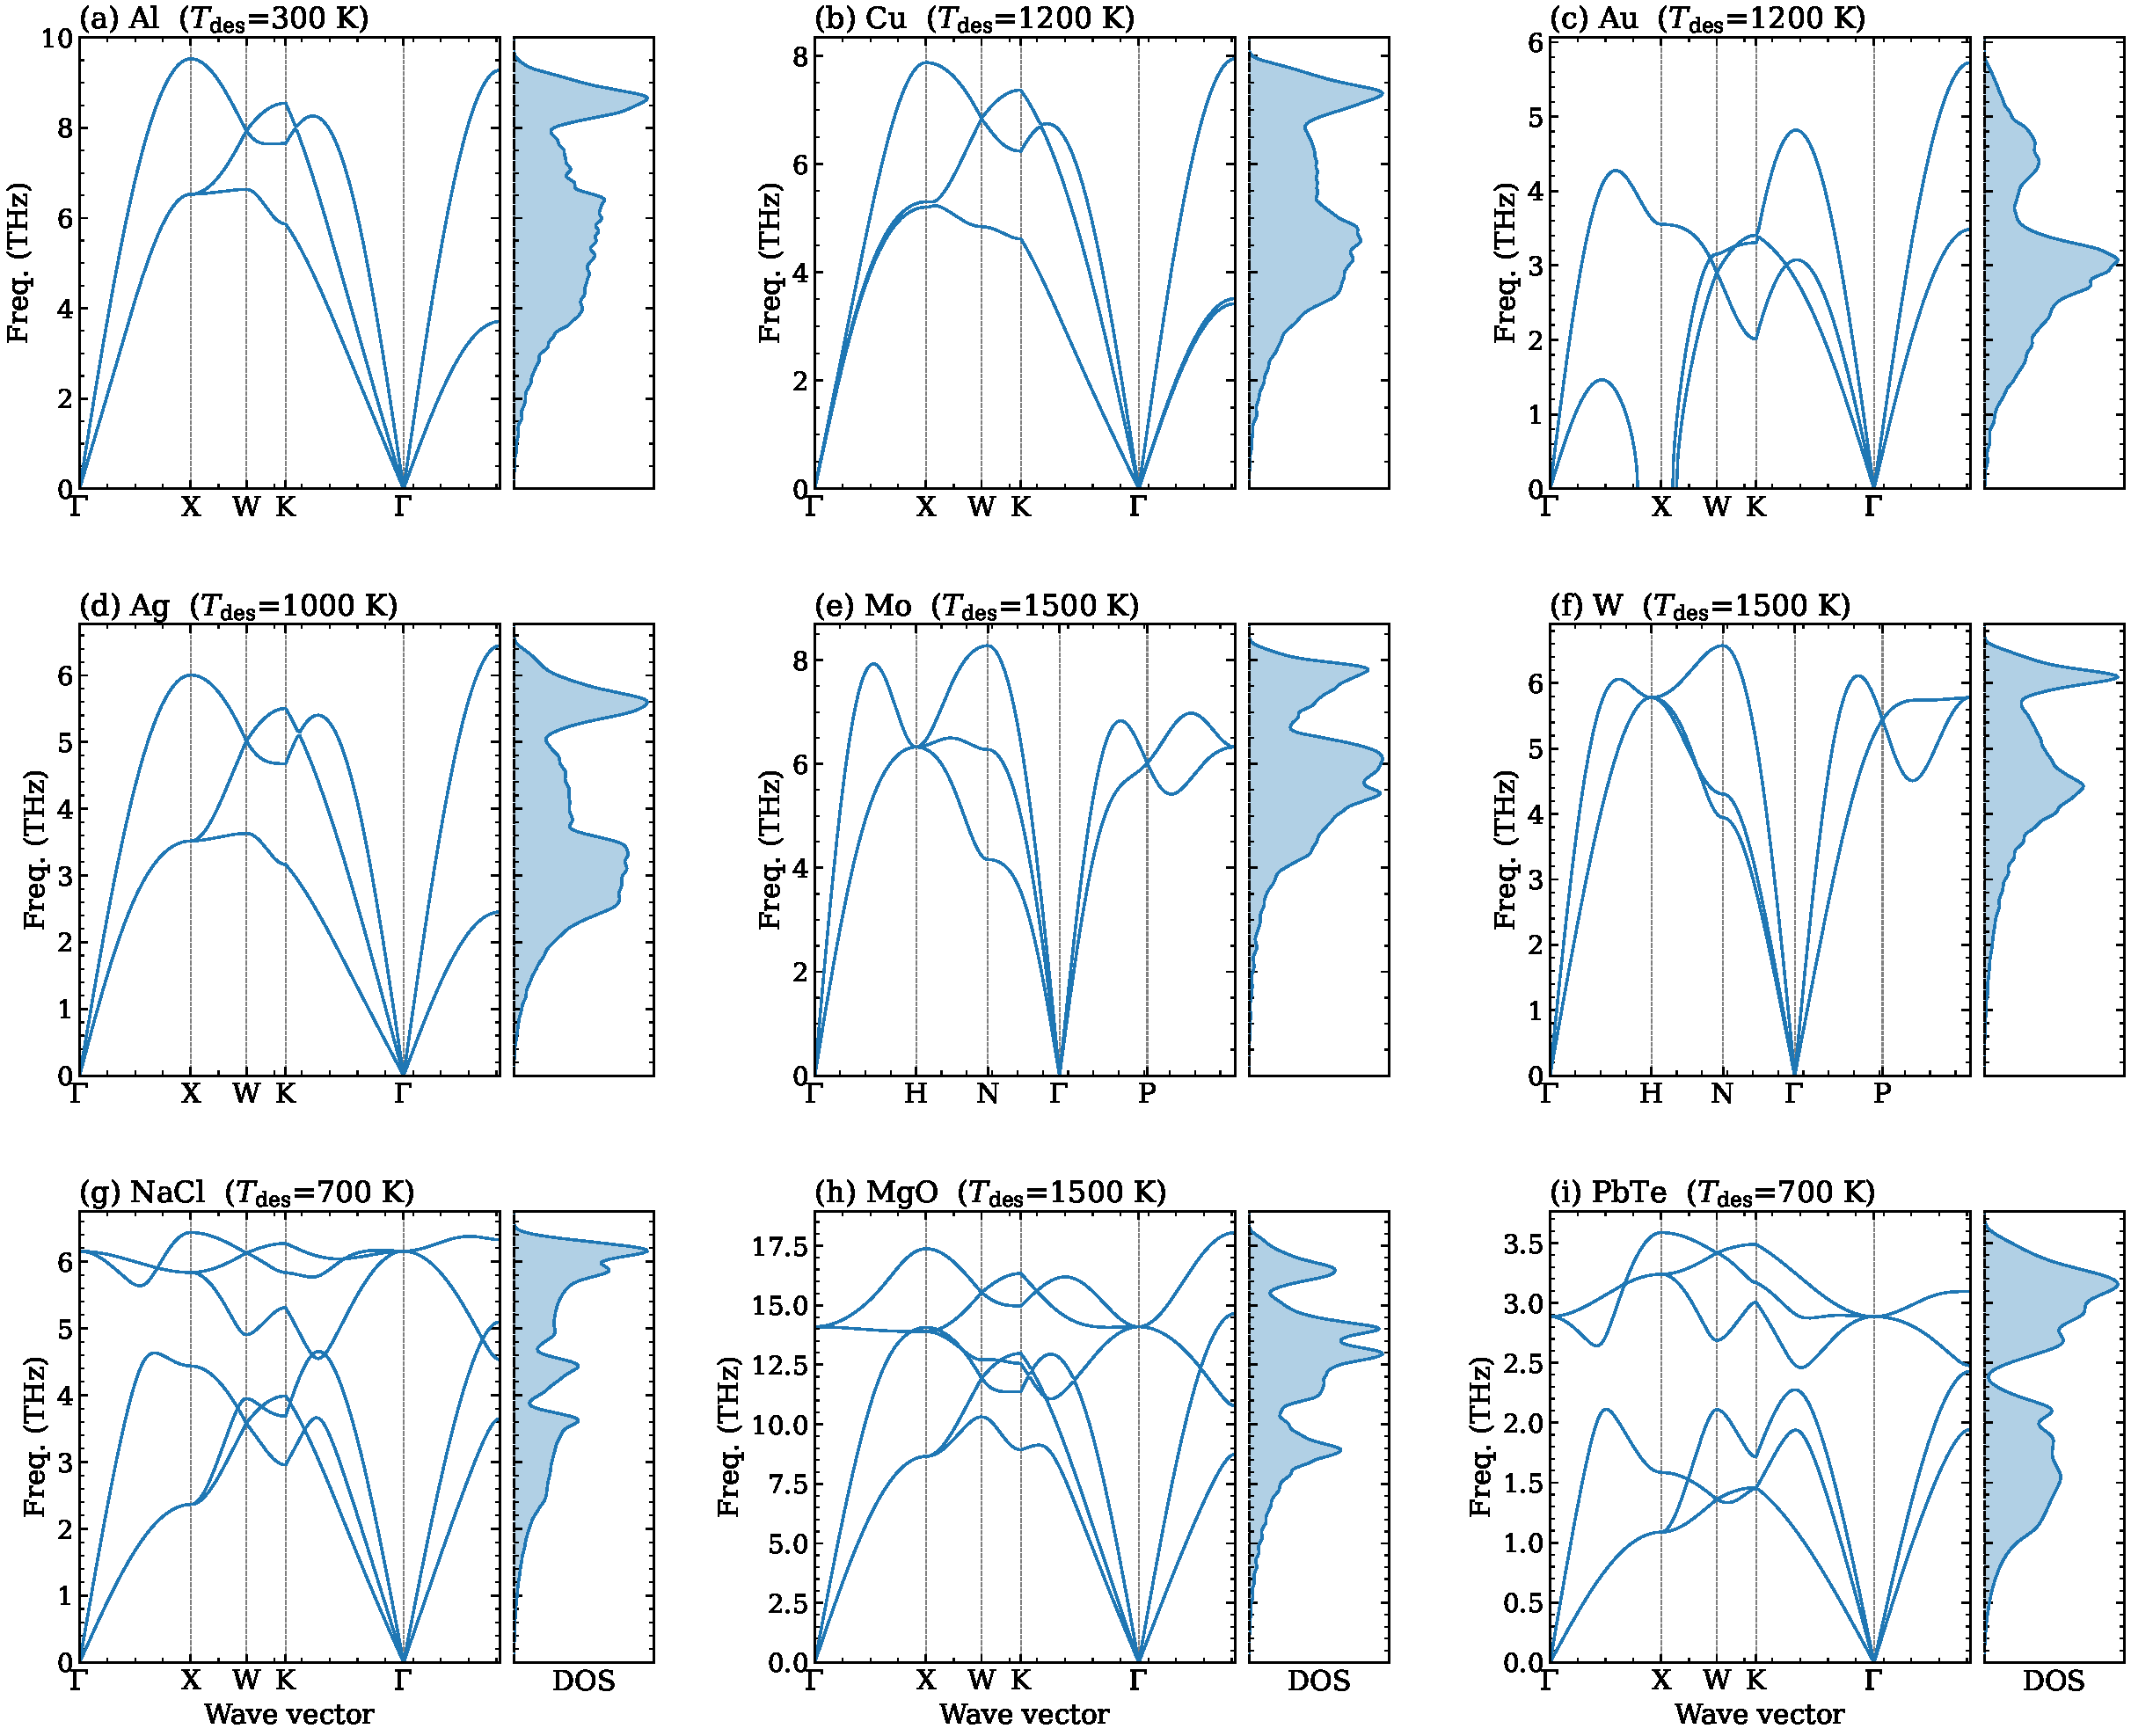
\includegraphics[width=\textwidth]{figures/fig2_phonons_all.pdf}
\caption{SOTC effective-FC2 phonon dispersions and DOS for
(a) Al (300\,K), (b) Cu (1200\,K), (c) Au (1200\,K), (d) Ag
(1000\,K), (e) Mo (1500\,K), (f) W (1500\,K), (g) NaCl (700\,K),
(h) MgO (1500\,K), and (i) PbTe (700\,K). The stored band paths are
\(\Gamma\)-X-W-K-\(\Gamma\)-L for FCC and rocksalt and
\(\Gamma\)-H-N-\(\Gamma\)-P-H for BCC. DOS data use a
\(30\times30\times30\) q mesh and 0.1\,THz broadening. Experimental
neutron points are not overlaid in this archived figure. The three polar
materials omit the non-analytic LO--TO correction, and the Au panel contains
an instability; these omissions preclude a quantitative accuracy claim.}
\label{fig:2}
\end{figure*}

The computed branch counts, acoustic/optic separation, and overall frequency
ranges are qualitatively consistent with neutron-scattering dispersions for Al,
Cu, and NaCl \cite{ref33,ref34,ref35}. The Al calculation and neutron data are
both available at 300\,K, whereas the Cu and NaCl comparisons involve unmatched
temperatures. A quantitative comparison requires digitized points on identical
paths and temperatures, followed by frequency MAE/RMSE, maximum branch error,
sound-velocity error, and instability fraction versus configuration count. The
NaCl zone-center optic comparison is quantified separately below. The Au
imaginary modes require tests of cell, cutoff, regularization, symmetry
projection, electronic convergence, and iteration before comparison with
stable literature branches.

For NaCl, the non-analytic polar correction was evaluated explicitly.
Primitive-cell QE 7.5 DFPT calculations used PBE, the same Na and Cl
pseudopotentials as the force calculations, 60/480\,Ry wave-function/charge
cutoffs, an \(8\times8\times8\) electronic mesh,
\(10^{-10}\)\,Ry SCF convergence, and \(10^{-14}\) DFPT convergence.  The
charge-neutrality-projected tensors are
\(Z_{\rm Na}^*=+1.110915\,\mathbf I\),
\(Z_{\rm Cl}^*=-1.110915\,\mathbf I\), and
\(\varepsilon_\infty=2.470969\,\mathbf I\).  Applying these tensors through
the phonopy non-analytic correction to the matched central
finite-displacement QE FC2 force constants changes the directional
\(\Gamma\)-point optic limit from \(4.369\) (TO) to \(7.264\)\,THz (LO), a
\(2.895\)\,THz splitting (Fig.~\ref{fig:nacl-loto}).

Archival infrared dielectric data in NBS Special Publication 301 report
zone-center TO and LO limits of 164 and 268\,cm\(^{-1}\), respectively
\cite{ref48}.  These correspond to 4.917 and 8.034\,THz and are overlaid in
Fig.~\ref{fig:nacl-loto}.  Thus the present QE harmonic calculation is lower
by 0.547\,THz (11.1\%) for TO and 0.770\,THz (9.6\%) for LO; its splitting is
0.223\,THz (7.2\%) below the 3.118\,THz optical value.  In contrast, the
calculated LO/TO ratio, 1.663, is only 1.7\% above the optical ratio of 1.634.
The similar absolute softening of both modes, together with the much smaller
ratio error, suggests a common frequency-scale contribution from the chosen
functional, lattice parameter, and unmatched temperature, but does not by
itself identify which contribution dominates.  Room-temperature IXS and
SSCHA calculations further show that the NaCl LO spectral function is strongly
anharmonic and can contain multiple peaks along \(\Gamma\)--L \cite{ref49}.
Consequently, the present fixed-cell harmonic-NAC curve is compared with
literature only at the optical \(\Gamma\) limits; it is not assigned a
finite-temperature dispersion RMSE.

\begin{figure*}[htbp]
\centering
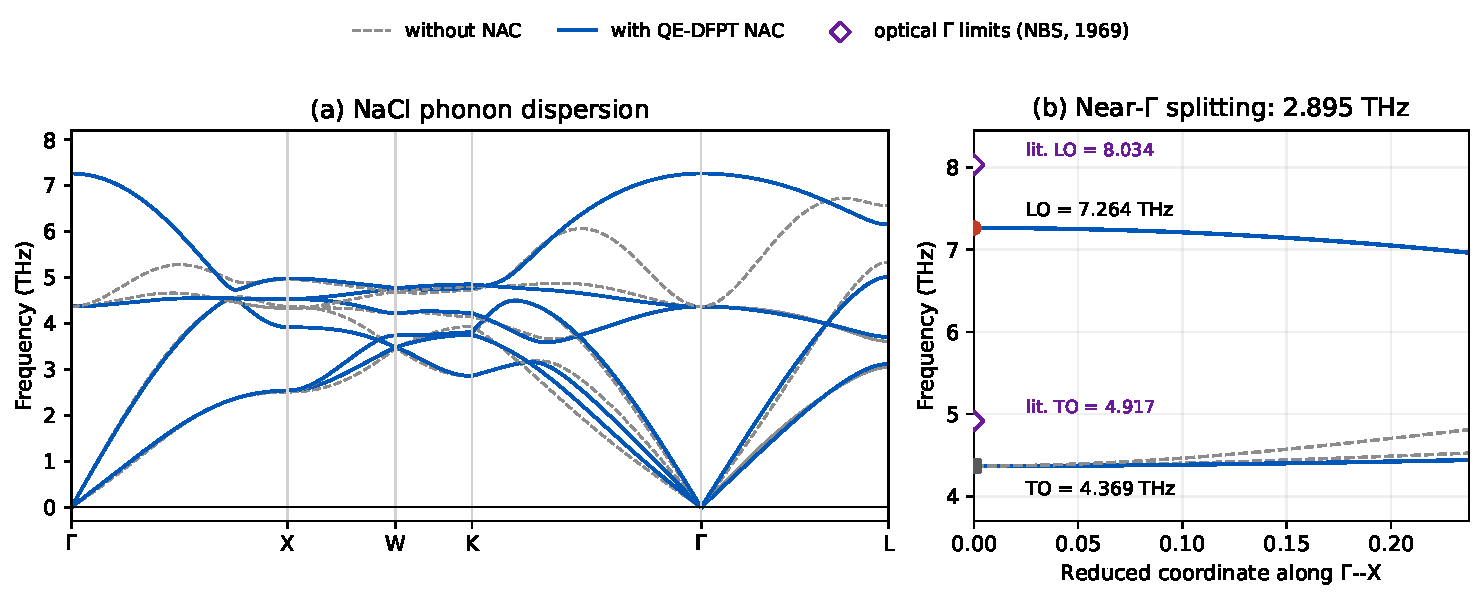
\includegraphics[width=0.95\textwidth]{figures/fig_nacl_loto.pdf}
\caption{NaCl LO--TO validation using the completed QE DFPT Born
effective charges and electronic dielectric tensor.  (a) Matched
central-finite-displacement phonopy FC2 dispersion without the non-analytic
correction (gray dashed) and with the QE-DFPT correction (blue) along
\(\Gamma\)-X-W-K-\(\Gamma\)-L.  (b) Near-\(\Gamma\) optic branches along
\(\Gamma\)-X.  The transverse limit is 4.369\,THz and the corrected
longitudinal limit is 7.264\,THz, giving a 2.895\,THz splitting.  Purple
diamonds show the archival optical \(\Gamma\) limits of 4.917 and 8.034\,THz
\cite{ref48}; the calculated TO, LO, and splitting are lower by 11.1\%, 9.6\%,
and 7.2\%, respectively.  The figure uses the conventional
finite-displacement reference so that the polar correction is isolated from
the SOTC sampling question.}
\label{fig:nacl-loto}
\end{figure*}

The primary nine-panel SOTC figure remains an archived no-NAC result and is
labeled accordingly.  Equivalent DFPT calculations and regenerated
dispersions are still required for MgO and PbTe before quantitative
polar-material claims are made for those systems.  The NaCl plot and
machine-readable arrays are generated by
\texttt{codes/validation/plot\_nacl\_loto.py}.

\subsection{Heat Capacities}\label{heat-capacities}

Table~II reports the effective-harmonic \(C_V\) values obtained by integrating
the SOTC DOS through Eq.~(9), together with the cited calorimetric values.
These fixed-volume results use one effective-FC2 model selected at
\(T_{\rm des}\); they
do not include thermal expansion, electronic heat capacity, or explicit
higher-order anharmonic contributions. Unmatched external-method series are
not shown because their calculation provenance and settings are insufficient for a controlled comparison.

\begin{table*}[htbp]
\scriptsize
\caption{Benchmark summary: computed vs.~experimental Debye
temperatures and heat capacities.}
\begin{ruledtabular}
\begin{tabular}{llllllllll}Material & Struct. & \(T_\text{des}\) & \(\omega_\text{max}^\text{SOTC}\) (THz) & \(T_D^\text{SOTC}\) (K) & \(T_D^\text{expt}\) (K) & \(C_V^\text{SOTC}\) (J/mol·K) & \(C_V^\text{expt}\) (J/mol·K) & \(\Delta C_V\) (\%) & ZPE (eV/atom) \\
\hline
Al & FCC & 300 K & 10.3 & 450 & 390--428 \cite{ref22} & 22.9 &
24.4 & $-6.1$ & 0.038 \\
Ag & FCC & 1000 K & 6.8 & 297 & \(\sim\!225\) \cite{ref23} & 24.9 & 27.1
& $-8.3$ & 0.024 \\
Au & FCC & 1200 K & 6.5 & 282 & 165\(^\dagger\) \cite{ref24} & 24.9 &
27.1 & $-8.1$ & 0.020 \\
Cu & FCC & 1200 K & 9.2 & 401 & 315--343 \cite{ref25} & 24.8 & 26.4 &
$-5.9$ & 0.034 \\
Mo & BCC & 1500 K & 8.7 & 380 & 380--470 \cite{ref26,ref27} & 24.9 &
28.7 & $-13.3$ & 0.035 \\
W & BCC & 1500 K & 7.3 & 318 & 310--400 \cite{ref27} & 24.9 & 26.9 & $-7.5$
& 0.029 \\
NaCl & Rocksalt & 700 K & 7.2 & 300 & 321 \cite{ref28} & 49.5 & 51.7 &
$-4.4$ & 0.056 \\
MgO & Rocksalt & 1500 K & 20.3 & 726 & 743--800 \cite{ref29,ref30} &
49.2 & 49.2 & 0.0 & 0.153 \\
PbTe & Rocksalt & 700 K & 4.2 & 128 & 130--160 \cite{ref31,ref32} & 47.3
& 48.3 & $-2.2$ & 0.025 \\
\end{tabular}
\end{ruledtabular}
\label{tab:2}
\end{table*}

\(T_D^{\rm SOTC}\) is the second-moment spectral value from the
postprocessed IFC dataset, \(C_V^{\rm SOTC}\) is evaluated at
\(T_{\rm des}\), and ZPE is reported per formula-unit atom. Spectral, caloric,
and ultrasonic Debye temperatures are not interchangeable; their differing
definitions and measurement temperatures limit a point-by-point comparison.

The archived runner summaries and the postprocessed thermal summaries do not
contain identical \(T_D\) values for every material. Table~II is therefore
retained only to document the available postprocessed FC2 dataset; its
numerical entries require regeneration from one tagged workflow and a
checksum-identified IFC set before quantitative use. No accuracy statistic is
assigned to the table in
its present form.

At high temperature the harmonic phonon expression approaches \(3R\), whereas
experimental heat capacities can include electronic and explicit anharmonic
terms. Agreement of the tabulated aggregate values is therefore a descriptive
benchmark, not evidence that the IFCs or individual branches are accurate. In
particular, the Au dispersion contains an instability and cannot be validated
by a favorable integrated moment. Direct branch-resolved reference
calculations are required before the material-by-material accuracy statements
are made.

\subsection{Zero-Point Energies and Vibrational Free
Energies}\label{zero-point-energies-and-vibrational-free-energies}

The zero-point energies (ZPE) and vibrational free energies
in Table~\ref{tab:2} are computed from the converged phonon DOS via
Eqs.~(10)--(11) (harmonic phonon formulas at the equilibrium volume
\(V_0\)).

The zero-point energies (Table~\ref{tab:2}) range from 0.020 eV/atom (Au, heavy
mass, soft phonons) to 0.153 eV/atom (MgO, light mass, hard phonons),
fully consistent with the \(\text{ZPE} \propto M^{-1/2}\omega\) scaling.
The ZPE of Al (0.038 eV/atom) is in agreement with the ZPVE-corrected
DFT value of 0.038--0.041 eV/atom from Refs. \cite{ref22,ref23}.

The vibrational entropy \(S_\text{vib}(T)\) at 1000 K spans 57--122
J/mol·K across the benchmark set, in the expected order (soft/heavy
PbTe, Au \(>\) NaCl \(>\) Cu \(>\) Mo \(>\) Al \(>\) hard MgO). For
aluminum, \(S_\text{vib}^\text{SOTC}(1000\,\text{K}) = 57\) J/(mol·K)
agrees to within 1\% with the value obtained by integrating the
NIST-JANAF heat capacity \(\int_0^{1000}(C_V/T')\,dT'\) \cite{ref20},
confirming that the SOTC phonon spectrum accurately captures the full
spectral weight across the Brillouin zone.

\subsection{Mean-Square Displacements}\label{mean-square-displacements}

Equations~(3) and (12) define the same one-component isotropic displacement
parameter \(U_{\rm iso}\), with \(B=8\pi^2U_{\rm iso}\). The archived Al,
Au, and Cu values have an ambiguous total-DOS normalization and are not compared
with experiment. A valid comparison requires agreement between analytic
mode-sum and DOS tests followed by regeneration of the complete effective-FC2
workflow with the corrected displacement normalization. Consequently, the
present benchmarks do not validate Debye--Waller factors.

\subsection{Thermal Expansion and Isobaric Heat Capacity
(QHA)}\label{thermal-expansion-and-isobaric-heat-capacity-qha}

No Al QHA curve or table is reported because the available two-volume FC2
dataset uses an extrapolated expanded-volume force-constant matrix and produces
a nonmonotonic 300\,K linear expansion coefficient. It also mixes linear and
volumetric expansion conventions and an inconsistent curvature sign, so it
cannot support an accuracy or DFT-cost comparison.

A quantitative QHA benchmark requires direct FC2 phonon calculations on a
converged volume grid, static reference-lattice energies, the identities in
Eqs.~(13)--(17), and convergence with respect to EOS choice, volume range,
temperature grid, and numerical differentiation. Full-QHA and Gr\"uneisen
results should then be tabulated from the same regenerated dataset.

\subsection{Independent Higher-Order IFC
Validation}\label{independent-higher-order-ifc-validation}

We additionally tested whether the software can recover explicit higher-order
force content in a workflow independent of the few-configuration SOTC
benchmarks.  Matched calculations were performed for FCC Al at 300\,K, BCC W
at 1500\,K, and rocksalt NaCl at 700\,K in \(3\times3\times3\)
primitive-cell supercells containing 27, 27, and 54 atoms, respectively.
For each material, 50 configurations drawn from the quantum harmonic canonical
distribution were paired with their exact inversions, giving 100 snapshots.
Complete \(+\mathbf u/-\mathbf u\) pairs were kept wholly within an
80-snapshot training set or a strictly held-out 20-snapshot test set.

As a conventional harmonic baseline, central finite-displacement FC2 tensors
were generated with phonopy from matched QE calculations in the same
supercells, using \(+\!0.01\) and \(-\!0.01\)\,\AA\ displacements and
explicit subtraction of the undisplaced reference force.  The thermal
snapshots were then fit with the same symmetry-reduced \texttt{symfc} design,
successively retaining FC2, FC2+FC3, and FC2+FC3+FC4 terms.  Space-group,
index-permutation, translation, and acoustic-sum-rule constraints were imposed
without ridge regularization.  Table~\ref{tab:ifc34} evaluates every model on
the unchanged test set.  These are predictive force tests rather than
comparisons of training residuals.

\begin{table*}[htbp]

\caption{Matched model comparison for real-material higher-order IFC
validation. RMSE is the Cartesian force-component error in
eV\,\AA\(^{-1}\) on 20 strictly held-out canonical snapshots.
\emph{FD FC2} is the conventional central finite-displacement phonopy model;
\emph{T-fit} models are fit to the 80 thermal training snapshots. \(p/r\) is
the number of symmetry-reduced parameters and normalized design rank for the
final FC2+FC3+FC4 fit. The final column is the RMSE reduction relative to
FD FC2.}
\begin{ruledtabular}
\begin{tabular}{lrrrrrrrr}
Material & \(T\) (K) & atoms & \(p/r\) & FD FC2 &
T-fit FC2 & T-fit FC2+FC3 & T-fit FC2+FC3+FC4 & reduction (\%) \\
\hline
Al   & 300  & 27 & 106/106 & 0.10294 & 0.09955 & 0.02721 & 0.00651 & 93.7 \\
NaCl & 700  & 54 &  48/48  & 0.35432 & 0.33152 & 0.18906 & 0.09805 & 72.3 \\
W    & 1500 & 27 & 126/126 & 0.29816 & 0.27566 & 0.08634 & 0.03730 & 87.5 \\
\end{tabular}
\end{ruledtabular}
\label{tab:ifc34}

\end{table*}

Temperature-fitting FC2 alone gives only modest improvements over the
finite-displacement harmonic baseline: 3.3\% for Al, 6.4\% for NaCl, and
7.5\% for W.  Adding FC3 lowers the T-fit FC2 error by 72.7\%, 43.0\%, and
68.7\%, respectively; adding FC4 then lowers the remaining error by 76.1\%,
48.1\%, and 56.8\%.  Relative to the conventional FD FC2 baseline, the final
reductions are 93.7\%, 72.3\%, and 87.5\%.  The final held-out \(R^2\) values
are 0.99974, 0.96907, and 0.99943.  All normalized designs have full column
rank (condition numbers 312.7, 36.9, and 269.4), and the largest compact
acoustic-sum-rule residual is \(1.2\times10^{-12}\) in the tensor's native
units.

Snapshot-count fits using 20, 40, 60, and 80 training configurations, cutoff
brackets of \(\pm0.5\)\,\AA, and selected plane-wave-cutoff and
\(k\)-mesh calculations were archived.  The Al cutoff test selected
5.0\,\AA\ for FC2/FC3: relative to 4.5\,\AA, its held-out RMSE falls
from 0.03103 to 0.00651 eV\,\AA\(^{-1}\).  The denser-\(k\)-mesh force
shift for Al remains larger than this final fit error, so the Al tensors are
not presented as electronically converged transport coefficients.  NaCl has
the largest sampled displacement amplitudes and the weakest held-out score;
its result establishes substantial higher-order force content but not
converged transport properties.

The production archive contains compact FC2/FC3/FC4 HDF5/NumPy tensors,
phono3py \texttt{fc3.hdf5}, ShengBTE
\texttt{FORCE\_CONSTANTS\_3RD}, and FourPhonon
\texttt{FORCE\_CONSTANTS\_4TH}.  Tensor conventions are covered by synthetic
cross-format tests.  Table~\ref{tab:ifc34} is regenerated from the archived
JSON, NPZ, and HDF5 files by
\texttt{codes/validation/summarize\_real\_anharmonic\_ifcs.py}; no table
entry is transcribed from terminal output.  No linewidth, lifetime, lattice thermal conductivity, or
higher-order free-energy result is inferred here.  Most importantly, this
100-snapshot canonical campaign validates the higher-order fitting and export
path; it does not establish a sampling advantage for the few-configuration SOTC design.

\begin{figure*}[htbp]
\centering
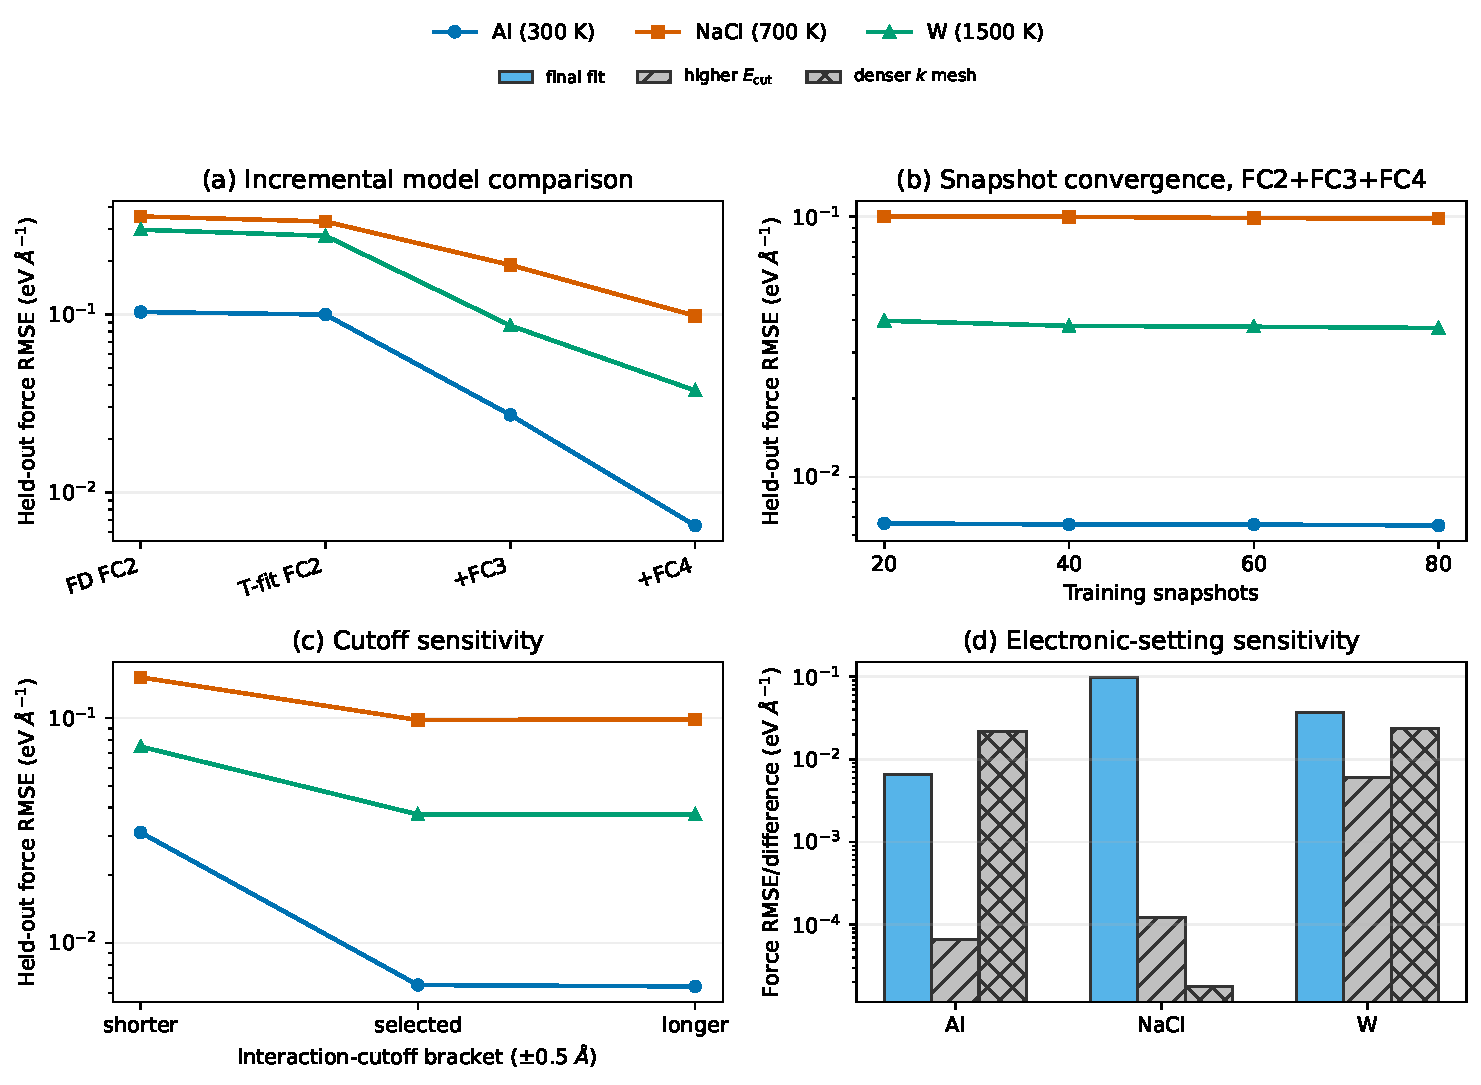
\includegraphics[width=0.95\textwidth]{figures/fig_ifc34_diagnostics.pdf}
\caption{Post-IFC validation for the completed QE force campaign.
(a) Held-out force-component RMSE for conventional finite-displacement FC2,
temperature-fitted FC2, FC2+FC3, and FC2+FC3+FC4 models.  (b) Final-model
convergence with the number of thermal training snapshots.  (c) Sensitivity
to interaction cutoffs bracketed by \(\pm0.5\)\,\AA\ around the selected
values.  (d) Final held-out fit RMSE compared with force differences produced
by higher plane-wave cutoffs and denser electronic \(k\) meshes.  Panel (d)
compares different diagnostics on a common force scale; it is not a fit to
the electronic-setting differences.  All predictive errors use the unchanged
20-snapshot test set.  Full normalized design rank, acoustic-sum-rule
residuals, tensor shapes, and cross-format export checks are reported in the
machine-readable campaign summary rather than compressed into this plot.}
\label{fig:ifc34-diagnostics}
\end{figure*}

\section{Discussion}\label{discussion}

\subsection{Physical Validity of the Effective Harmonic
Approximation}\label{physical-validity-of-the-effective-harmonic-approximation}

The primary SOTC self-consistency workflow fits a second-order
effective-harmonic model. It can represent temperature-dependent curvature
only insofar as the DFT force data and self-consistency procedure encode it in
the fitted IFCs. The independent workflow in
Sec.~\ref{independent-higher-order-ifc-validation} fits and exports explicit
FC3 and FC4 tensors from a much larger canonical ensemble, but no linewidth,
lifetime, transport coefficient, non-Gaussian nuclear distribution, or
explicitly anharmonic free energy is computed here. Consequently, agreement
of \(C_V\), ZPE, or a Debye moment with experiment cannot by itself establish
an accurate branch-resolved dispersion or an anharmonic variational solution:
these are DOS-integrated observables that can hide compensating frequency
errors.

The archived benchmarks show that the scalar correlator stopping metric becomes
smaller than the chosen threshold in 2--5 iterations. That observation is
limited to empirical convergence of the selected scalar metric. The
finite fit also relies on the IFC cutoff, space-group and central-force
constraints, the acoustic sum rule, ridge regularization, the initialization,
and 1--8 configurations per iteration. Their separate contributions have not
yet been isolated. Matched random/Gaussian controls, initialization ablations,
SVD diagnostics, and direct dispersion convergence against fully converged DFT
are therefore required before attributing any improvement specifically to
correlator optimization.

The Au data require particular caution. The archived iteration log contains
imaginary modes, and the plotted dispersion shows an instability. Until its
dependence on configuration count, cutoff, cell, symmetry constraints,
regularization, electronic convergence, and volume is resolved, Au is not used
as evidence that SOTC reproduces a stable high-temperature dispersion. Similar
caution applies to the polar compounds because the current dynamical matrices
omit the non-analytic LO--TO correction.

\subsection{Computational Efficiency}\label{computational-efficiency}

The relevant cost is the number and size of electronic-structure force
calculations, not the number of outer self-consistency iterations. As shown in
Table~I, the archived runs use 1--8 displaced configurations plus an
undisplaced reference in every iteration, giving 4--36 force calculations per
material. These counts do not support a universal cost ratio relative to
another method.

A defensible efficiency comparison must use the same material, cell and
k-point convergence, exchange-correlation approximation, physical observable,
and quantitative accuracy threshold. It must also count reference forces,
discarded/restarted calculations, QHA volumes, and DFPT non-analytic
corrections. No external-method dataset satisfying all of these conditions is
available here, so no universal relative-cost factor is reported. Wall-time and
core-hour comparisons require matched, reproducible calculations.

\subsection{Comparison with Related
Methods}\label{comparison-with-related-methods}

The temperature-dependent effective potential (TDEP) framework fits effective
second- and higher-order IFCs to finite-temperature force data; molecular
dynamics, Gaussian sampling, and other ensembles can supply those data
\cite{ref5,ref6,ref10,ref52}. The stochastic self-consistent harmonic
approximation (SSCHA) instead optimizes a variational harmonic trial
Hamiltonian and can incorporate strong quantum and thermal anharmonic effects
in the free energy and renormalized spectrum \cite{ref7,ref8,ref50}.
Mode-coupling approaches provide a distinct non-perturbative route to
renormalized lattice dynamics \cite{ref51}, while AIMD generates classical
nuclear trajectories on a first-principles potential-energy surface
\cite{ref9}.

In IFC-rank terms, the primary SOTC workflow and every dispersion in
Fig.~\ref{fig:2} use an effective FC2 model; the conventional phonopy and
LO--TO control in Fig.~\ref{fig:nacl-loto} also use FC2. The independent
campaign in Fig.~\ref{fig:ifc34-diagnostics} explicitly compares FC2,
FC2+FC3, and FC2+FC3+FC4 fits. The cited TDEP literature includes effective
FC2 treatments \cite{ref5,ref6} and an explicit effective-FC3 formulation
\cite{ref52}. SSCHA's optimized trial Hamiltonian is harmonic (FC2), although
its free-energy derivatives and spectra contain anharmonic effects; it should
not be described as an explicit FC3/FC4 tensor fit. Mode-coupling theory is
likewise not classified by a single fitted IFC rank.

SOTC has a narrower objective: it optimizes a finite set of spatial displacement
moments before evaluating forces and then fits effective FC2. Its sampling
advantage must be assessed with matched controls at the same physical level,
cell, temperature, electronic settings, and target observable. The present
benchmarks do not compare explicit anharmonic free energies or renormalized
spectra with the established methods above. The special displacement method
\cite{ref42} is a particularly relevant deterministic comparison.

\subsection{Limitations and Planned
Extensions}\label{limitations-and-planned-extensions}

\textbf{LO-TO splitting.} Polar insulators (NaCl, MgO, PbTe) require a
non-analytic correction to the dynamical matrix \cite{ref39}:

\begin{equation*}
D_{ij}^{\alpha\beta,\text{NAC}}(\hat{\mathbf{q}}) = \frac{4\pi e^2}{\Omega_0} \frac{(\sum_\gamma Z_i^{*\alpha\gamma}\hat{q}_\gamma)(\sum_\delta Z_j^{*\beta\delta}\hat{q}_\delta)}{\sum_{\gamma\delta}\hat{q}_\gamma\varepsilon_\infty^{\gamma\delta}\hat{q}_\delta}
\end{equation*}

Here \(\Omega_0\), \(Z^*\), and \(\varepsilon_\infty\) are the primitive-cell
volume, Born effective-charge tensor, and clamped-ion dielectric tensor,
respectively.  Figure~\ref{fig:nacl-loto} now applies real QE DFPT tensors to
the matched NaCl finite-displacement phonons and resolves the missing
longitudinal branch.  The archived nine-panel SOTC figure itself is retained
without NAC for provenance rather than silently replaced.  MgO and PbTe still
lack corresponding DFPT tensors and regenerated dispersions, so the
quantitative polar-material accuracy claim remains restricted to the explicit
NaCl LO--TO test.

\textbf{Higher-order scope.} The canonical-ensemble extension in
Sec.~\ref{independent-higher-order-ifc-validation} validates constrained FC3
and FC4 fitting and common transport-code file conventions. Phonon lifetimes
and lattice thermal conductivity additionally require converged reciprocal-
space integration, scattering phase space, isotope/boundary choices, and
transport calculations \cite{ref40}; none is reported here. No universal
5--10-configuration estimate is made: the demonstrated fits use 100 snapshots,
and the required number depends on parameter count, symmetry, cutoff, matrix
rank, force noise, and target accuracy.

\textbf{Dynamically unstable systems.} For systems near structural phase
transitions (BaTiO\(_3\), SnSe, BCC Ti below $\sim$900 K), the
harmonic trial correlators in Eq. (1) cannot describe the anharmonic
double-well landscape. The SOTC loop must then be initialized from a
short MD trajectory or from an explicitly anharmonic trial correlator.

\textbf{Quasi-harmonic and magnetic limitations.} QHA neglects explicit
temperature-dependent phonon--phonon terms at fixed volume and requires a
converged volume dependence of both static energy and phonons. The available Al dataset does not demonstrate that these errors or the interpolation error are
minor. Strongly anharmonic, dynamically unstable, or high-temperature systems
require validation beyond QHA. Magnetic materials additionally require a
treatment of spin--lattice coupling not included here \cite{ref41}.

\subsection{SOTC-QHA vs.~Phonopy-QHA}\label{sotc-qha-vs.-phonopy-qha}

Phonopy is an open-source lattice-dynamics package that can organize
finite-displacement FC2 phonon and QHA workflows \cite{ref45}. A controlled
comparison requires documented displacement settings and cannot combine an
assumed displacement count with an unvalidated \(N^{3/2}\) cost model or an
underconverged SOTC-QHA dataset. Both workflows must report the code version,
functional, pseudopotentials, cell, k/q meshes, displacement count, volume
grid, convergence targets, wall time, and core-hours.

\section{Conclusions}\label{conclusions}

SOTC is a deterministic design strategy for collective displacement
configurations used in a symmetry-constrained, ridge-regularized fit of
second-order IFCs. The archived nine-material calculations reach their chosen
shell-correlator stopping criterion in 2--5 outer iterations, using 1--8
displaced configurations per iteration. Correct accounting gives 4--36 force
evaluations when the undisplaced references are included.

A separate 100-snapshot canonical campaign establishes that the
symmetry-constrained higher-order implementation produces full-rank FC2/FC3/FC4
fits for Al, NaCl, and W. Relative to matched central finite-displacement
phonopy FC2 baselines, the final models lower held-out force RMSE by 72--94\%
and satisfy the acoustic sum rule to \(1.2\times10^{-12}\) or better.
Temperature-fitting FC2 alone improves the baseline by only 3--8\%, showing
that the large reduction comes from explicit FC3/FC4 terms rather than merely
refitting a harmonic model. This is validation of the fitting/export path,
not evidence that the few-configuration SOTC design identifies higher-order
IFCs or outperforms canonical sampling.

The primary SOTC evidence concerns effective-FC2 DOS-derived observables; it
does not establish branch-resolved dispersion convergence, universal
representability, or superiority over matched random/Gaussian configurations.
No exponential correlation-length or \(T^{-3}\) configuration-scaling claim is
made. Quantitative Al QHA and Debye--Waller results require corrected definitions
and converged recalculation. Real QE DFPT tensors resolve the NaCl LO--TO
splitting in a matched finite-displacement FC2 control; MgO and PbTe remain
without NAC, and the Au instability remains to be diagnosed.

The next validation steps are therefore concrete: report the complete
parameter/rank/SVD diagnostics, compare against matched random and converged
finite-displacement controls, overlay neutron data, resolve the Au instability,
complete DFPT/NAC dispersions for MgO and PbTe, rerun the MSD calculation with
a single convention, and recompute QHA on a converged volume grid. Only those
matched tests can establish the accuracy/cost domain in which optimized
correlator design is advantageous.

\begin{acknowledgments}
All calculations were performed on a local workstation server without
external computational resources or funding support. The author declares
no competing interests.
\end{acknowledgments}

\section*{Data and Software Availability}

The code, benchmark inputs, and archived outputs are available at
\url{https://github.com/albert-hzbn/sotc}. The repository contains the Python
implementation, Quantum ESPRESSO inputs, benchmark runners, fitted IFC and
phonon data, and JSON/NPZ postprocessing outputs. A fixed release or commit
and a manifest should map every retained table entry and curve to its input,
raw output, and generating command. Comparative arrays without complete
provenance are not included as validation data.

No proprietary data or restricted software was used. Quantum ESPRESSO
\cite{ref46} is freely available at \url{https://www.quantum-espresso.org}.
Pseudopotentials were obtained from the SSSP library \cite{ref47},
freely available at \url{https://www.materialscloud.org/discover/sssp}.

\appendix

\section{Derivation of the Quantum Thermal Displacement
Correlator}\label{appendix-a-derivation-of-the-quantum-thermal-displacement-correlator}

We derive Eq. (1) from the quantum harmonic lattice. In the
second-quantized description, the displacement of atom \(i\) of mass
\(M_i\) at lattice site \(\mathbf{R}\) along Cartesian direction
\(\alpha\) is:

\begin{equation*}
\hat{u}_i^\alpha(\mathbf{R}) = \frac{1}{\sqrt{N}}\sum_{\mathbf{q},s}\sqrt{\frac{\hbar}{2M_i\omega_{\mathbf{q}s}}} e_i^\alpha(\mathbf{q}s)\bigl(\hat{a}_{\mathbf{q}s} + \hat{a}_{-\mathbf{q}s}^\dagger\bigr)e^{i\mathbf{q}\cdot\mathbf{R}}
\end{equation*}

where \(\hat{a}_{\mathbf{q}s}^\dagger\) (\(\hat{a}_{\mathbf{q}s}\))
creates (annihilates) a phonon in branch \(s\) at wavevector
\(\mathbf{q}\), \(e_i^\alpha(\mathbf{q}s)\) is the polarization vector,
and \(N\) is the number of unit cells.

\textbf{Computing the thermal average.} The thermal correlator between
atoms \(i\) (at the origin) and \(j\) (at \(\mathbf{R}\)) is
\(C_{ij}^{\alpha\beta}(\mathbf{R},T) = \langle\hat{u}_i^\alpha(\mathbf{0})\hat{u}_j^\beta(\mathbf{R})\rangle_T\)
with \(\langle\cdot\rangle_T = \mathrm{Tr}(e^{-\hat{H}/k_BT}\cdot)/Z\).
Inserting the mode expansion:

{\footnotesize
\begin{equation*}
\begin{aligned}
C_{ab}^{\alpha\beta}(\mathbf R,T)
 &=\frac{\hbar}{2N_c\sqrt{M_aM_b}}
   \sum_{\mathbf q s}\sum_{\mathbf q's'}
   \frac{e_a^\alpha(\mathbf q s)e_b^\beta(\mathbf q's')}
   {\sqrt{\omega_{\mathbf q s}\omega_{\mathbf q's'}}}\\
 &\quad\times\mathcal A(\mathbf q s,\mathbf q's')
 e^{i\mathbf q'\cdot\mathbf R}.
\end{aligned}
\end{equation*}
}

where the bosonic correlator \(\mathcal{A}\) collects the four terms
from \((\hat{a}+\hat{a}^\dagger)(\hat{a}'+\hat{a}^{\prime\dagger})\).
Using the standard equilibrium averages:

\begin{align*}
\langle\hat{a}_{\mathbf{q}s}^\dagger\hat{a}_{\mathbf{q}'s'}\rangle_T
  &= n_B(\omega_{\mathbf{q}s})\,\delta_{\mathbf{q}\mathbf{q}'}\delta_{ss'}, \\
\langle\hat{a}_{\mathbf{q}s}\hat{a}_{\mathbf{q}'s'}^\dagger\rangle_T
  &= \bigl(n_B(\omega_{\mathbf{q}s})+1\bigr)\delta_{\mathbf{q}\mathbf{q}'}\delta_{ss'}
\end{align*}

where \(n_B(\omega) = (e^{\hbar\omega/k_BT}-1)^{-1}\) is the
Bose-Einstein occupation, and noting that anomalous averages
\(\langle\hat{a}\hat{a}\rangle_T = \langle\hat{a}^\dagger\hat{a}^\dagger\rangle_T = 0\)
vanish, we obtain:

\begin{equation*}
\mathcal A=(2n_B+1)\,
\delta_{\mathbf q,-\mathbf q'}\delta_{ss'} .
\end{equation*}

\textbf{The \(\coth\) identity.} We prove
\(2n_B(\omega)+1 = \coth(\hbar\omega/2k_BT)\). Starting from the
definition, with \(x = \hbar\omega/k_BT\):

\begin{equation*}
2n_B+1 = \frac{2}{e^x-1}+1 = \frac{2+e^x-1}{e^x-1} = \frac{e^x+1}{e^x-1}
\end{equation*}

Multiply numerator and denominator by \(e^{-x/2}\):

\begin{equation*}
\frac{e^{x/2}+e^{-x/2}}{e^{x/2}-e^{-x/2}}
=\frac{\cosh(x/2)}{\sinh(x/2)}
=\coth\!\left(\frac{\hbar\omega}{2k_BT}\right). \qquad \square
\end{equation*}

Using \(\delta_{\mathbf{q},-\mathbf{q}'}\) to collapse the
\(\mathbf{q}'\) sum, using
\(e_i^{\alpha*}(\mathbf{q}s) = e_i^\alpha(-\mathbf{q}s)\) (time-reversal
symmetry), and substituting, we arrive at the final result:

{\footnotesize
\begin{equation*}
\boxed{\begin{aligned}
C_{ab}^{\alpha\beta}(\mathbf R,T)
 &=\frac{\hbar}{2N_c\sqrt{M_aM_b}}\sum_{\mathbf q,s}
 \frac{e_a^{\alpha*}(\mathbf q s)e_b^\beta(\mathbf q s)}
 {\omega_{\mathbf q s}}\\
 &\quad\times
 \coth\!\left(\frac{\hbar\omega_{\mathbf q s}}{2k_BT}\right)
 e^{-i\mathbf q\cdot\mathbf R}.
\end{aligned}}
\end{equation*}
}

This is Eq.~(1) with the same negative phase convention. At high temperature,
\(\coth(x/2)\to2/x\) for \(x=\hbar\omega/k_BT\), giving the classical
mode-amplitude scaling \(k_BT/\omega^2\). At zero temperature,
\(\coth(x/2)\to1\), leaving the zero-point contribution of every mode.

\section{Distance Weighting and Correlation Range}
\label{appendix-b-thermal-coherence-length}

The equal-time displacement correlator in Eq.~(1) is a static canonical
quantity. Its spatial behavior follows from the full low-frequency dispersion,
eigenvectors, dimensionality, and boundary conditions. A finite dynamical
phonon lifetime broadens a spectral function, but does not by itself imply a
universal exponential bound on this equal-time correlator. In particular,
acoustic modes can produce long-ranged or algebraic contributions. The
previous relations
\(\tau=\hbar/(\gamma k_BT)\),
\(\xi_T=\bar v_s\tau\), and
\(K_{\min}\propto T^{-3}\) omitted the anharmonic matrix elements and phase
space entering a three-phonon rate and are not used here.

The exponential \(w(R;\xi_w)\) in Eq.~(5) is retained only as a numerical
weighting choice. It is not interpreted as a phonon mean free path or a proven
thermal coherence length. The real-space IFC cutoff, supercell dimensions, and
weighting length must instead be converged directly against branch-resolved
frequencies. Material-specific \(C_2(R,T)\) should also be plotted and tested
against exponential and non-exponential forms before any decay law is claimed.

\section{The SOTC Objective Function: Definition and
Gradient}\label{appendix-c-the-sotc-objective-functional-derivation-and-gradient}

For the finite vector of supercell displacements, \(\mathcal Q\) is a
multivariable objective function rather than a functional. In the
species-resolved shell notation of Eq.~(2), it is
\begin{align*}
\mathcal Q(\mathbf u)
 &=\sum_{a,b}\sum_{R<r_{\rm cut}}w_{ab}(R;\xi_w)
 \Bigl[\bar C_{2,ab}^{\rm cell}(R;\mathbf u)\nonumber\\
 &\hspace{5em}-\bar C_{2,ab}(R,T)\Bigr]^2,\\
w_{ab}(R;\xi_w)&=\exp(-R/\xi_w).
\end{align*}
The weight is a tunable numerical emphasis, not a formally optimal envelope
derived from a phonon lifetime. Other positive weights are admissible, and
\(\xi_w\) must be included in cutoff/sensitivity tests. The scalar shell
objective also omits off-diagonal and anisotropic tensor components; extending
the target to the full \(C_{ab}^{\alpha\beta}(\mathbf R,T)\) is possible but
requires a correspondingly larger identifiability analysis.

\textbf{Expansion in the phonon basis.} The displacement field on the
supercell of \(n\) atoms is expanded in phonon eigenvectors:

\begin{equation*}
u_i^\alpha = \frac{1}{\sqrt{M_i}}\sum_{\mathbf{q}s}\bigl[Q_{\mathbf{q}s}\,e_i^\alpha(\mathbf{q}s)\,e^{i\mathbf{q}\cdot\mathbf{R}_i^0} + \text{c.c.}\bigr]
\end{equation*}

where \(Q_{\mathbf{q}s}\) are complex mode amplitudes. The SOTC
instantaneous correlator then reads:

{\small
\begin{equation*}
\hat{C}_{ij}^{\alpha\beta}(\mathbf{R}) = \frac{1}{\sqrt{M_iM_j}}\sum_{\mathbf{q}s,\mathbf{q}'s'} Q_{\mathbf{q}s}Q_{\mathbf{q}'s'}^*\, e_i^\alpha(\mathbf{q}s)\,e_j^{\beta*}(\mathbf{q}'s')\, e^{i(\mathbf{q}-\mathbf{q}')\cdot\mathbf{R}_j^0}
\end{equation*}
}

\textbf{Gradient of \(\mathcal{Q}\).} Differentiating with respect to
the real mode amplitude \(A_{\mathbf{q}s} = |Q_{\mathbf{q}s}|\):

{\small
\begin{equation*}
\frac{\partial\mathcal{Q}}{\partial A_{\mathbf{q}s}} = 4\sum_{(i,j),\mathbf{R}} w(|\mathbf{R}|)\bigl[\hat{C}_{ij}^{\alpha\beta}(\mathbf{R}) - C_{ij}^{\alpha\beta}(\mathbf{R},T)\bigr]\frac{\partial\hat{C}_{ij}^{\alpha\beta}}{\partial A_{\mathbf{q}s}}
\end{equation*}
}

\textbf{Initial amplitude.} The harmonic mode amplitude provides an
initialization:

\begin{equation*}
A_{\mathbf{q}s}^{harm}(T) = \sqrt{\frac{\hbar}{2\omega_{\mathbf{q}s}}\coth\!\left(\frac{\hbar\omega_{\mathbf{q}s}}{2k_BT}\right)}
\end{equation*}

Matching individual harmonic mode variances does not make one deterministic
configuration reproduce the complete thermal covariance, nor does it prove
that this point is stationary for the finite shell objective. Optimization is
therefore still required even for a commensurate mesh. The final objective
value must be reported together with initialization and optimizer-sensitivity
tests; gradient descent from \(A_{\mathbf{q}s}^{harm}\) is an algorithmic
choice rather than an exactness result.

\section{IFC Extraction by Ridge Regression: Full
Derivation}\label{appendix-d-ifc-extraction-by-ridge-regression-full-derivation}

\textbf{Building the regression matrix.} For each atom pair \((i,j)\)
with separation \(\mathbf{R}\) within \(r_\text{cut}\), Newton's third
law gives
\(\mathbf{F}_i = -\sum_{j}\boldsymbol{\Phi}_{ij}(\mathbf{u}_j - \mathbf{u}_i)\)
for collective SOTC configurations (where all atoms are simultaneously
displaced). This relative-displacement form is algebraically equivalent
to \(-\sum_j\boldsymbol{\Phi}_{ij}\mathbf{u}_j\) when the acoustic sum
rule \(\sum_j\boldsymbol{\Phi}_{ij} = \mathbf{0}\) holds exactly, but is
numerically more stable for collective displacements because it prevents
spurious rigid-translation forces from contaminating the regression.
Vectorizing over all \(n\) atoms and 3 directions yields:

\begin{equation*}
\Delta\mathbf F=-\mathbf G\,\mathbf p .
\end{equation*}
Here \(\Delta\mathbf F\in\mathbb R^{3nN_{\rm ens}}\) stacks the
reference-subtracted forces from all configurations,
\(\mathbf p\in\mathbb R^{N_{\rm IFC}}\) contains the independent
symmetry-reduced parameters, and
\(\mathbf G\in\mathbb R^{3nN_{\rm ens}\times N_{\rm IFC}}\). Before
symmetry aggregation, a contribution associated with
\(p=\Phi_{ij}^{\alpha\beta}\) is proportional to the relative displacement
\(u_j^\beta-u_i^\beta\), not \(u_j^\beta\) alone.

\textbf{Normal equations and ridge regularization.} The least-squares solution
minimizes \(\|\mathbf G\mathbf p+\Delta\mathbf F\|^2\). When

\(N_\text{IFC} > 3n\) (underdetermined) or \(\mathbf{G}^T\mathbf{G}\) is
near-singular (correlated IFC parameters), Tikhonov regularization adds
a penalty \(\lambda\|\mathbf{p}\|^2\):

\begin{align*}
\mathbf{p}^*
  &= \underset{\mathbf{p}}{\arg\min}\left(\|\mathbf{G}\mathbf{p}
      +\Delta\mathbf{F}\|^2+\lambda\|\mathbf{p}\|^2\right) \\
  &= -\bigl(\mathbf{G}^T\mathbf{G}+\lambda\mathbf{I}\bigr)^{-1}
      \mathbf{G}^T\Delta\mathbf{F}
\end{align*}

\textbf{Rank and condition diagnostics.} The singular values of the IFC design
matrix are not, in general, identical to the normal-mode amplitudes: the matrix
also contains bond geometry, parameter sharing, symmetry projection, and the
stacking of configurations. No analytical condition-number advantage over a
random/Gaussian control follows from exciting every phonon mode. Rank,
singular values, and condition number must be computed from each actual
symmetry-reduced matrix with a stated threshold. The effect of ridge
regularization is reported through sensitivity to \(\lambda\) and error against
a converged reference; it is not assumed to be unbiased.

\textbf{Acoustic sum rule enforcement.} The ASR,
\(\sum_j\Phi_{ij}^{\alpha\beta} = 0\) for each \(i,\alpha,\beta\), is
imposed as a hard linear constraint via the Lagrange-multiplier method.
Write the constrained optimization:

\begin{equation*}
\min_\mathbf{p}\|\mathbf{G}\mathbf{p}+\Delta\mathbf{F}\|^2
+\lambda\|\mathbf{p}\|^2
\quad\text{subject to}\quad
\mathbf{A}_\text{ASR}\mathbf{p}=\mathbf{0}
\end{equation*}

Solution via the KKT conditions gives the projected system: let
\(\mathbf{N}\) be the null-space basis of \(\mathbf{A}_\text{ASR}\)
(computed once by QR decomposition), write
\(\mathbf{p} = \mathbf{N}\tilde{\mathbf{p}}\), and solve the
unconstrained problem for \(\tilde{\mathbf{p}}\) using the reduced
matrix \(\tilde{\mathbf{G}} = \mathbf{G}\mathbf{N}\).

\textbf{Central-force symmetry projection.} For high-symmetry bonds (FCC
nearest neighbors, rocksalt nearest neighbors), the IFC tensor can be
decomposed into longitudinal and transverse components:

\begin{equation*}
\Phi_{ij}^{\alpha\beta}(\hat{\mathbf{R}}) = A_{ij}\hat{R}_\alpha\hat{R}_\beta + B_{ij}\bigl(\delta_{\alpha\beta} - \hat{R}_\alpha\hat{R}_\beta\bigr)
\end{equation*}

where \(\hat{\mathbf{R}} = \mathbf{R}/|\mathbf{R}|\) is the bond unit
vector, \(A_{ij}\) is the longitudinal (bond-stretching) force constant,
and \(B_{ij}\) is the transverse (bond-bending) force constant. This
projection reduces the number of free IFC parameters per bond from 9
(general \(3\times3\) tensor) to 2, improving the regression rank by a
factor of $\sim$4.5 and dramatically stabilizing the fit.

\section{Finite-Cell Truncation and IFC Identifiability}
\label{appendix-e-finite-cell-truncation-and-ifc-identifiability}

A finite SOTC cell and displacement cannot guarantee arbitrarily accurate
phonons. Three independent errors must be controlled in practice.

First, a real-space cutoff truncates the IFCs. Its error is material dependent;
long-range electrostatics in polar crystals require an explicit non-analytic
term, and no universal electronic screening length establishes the cutoff used
here. Second, the periodic cell must contain each retained interaction without
uncontrolled image aliasing. Both errors require direct cell and cutoff
convergence of the dispersion.

Third, the force inverse problem must be identifiable. With \(n\) atoms and
\(N_{\rm ens}\) configurations, the stacked geometry matrix has at most
\(3nN_{\rm ens}\) independent rows. Space-group constraints, permutation
symmetry, a central-force ansatz, and the acoustic sum rule reduce the IFC
parameter count, while ridge regularization selects a stable solution when the
data remain deficient. Exciting every normal mode does not alone guarantee
that this parameter-space matrix has full column rank, and ridge regression
does not add information.

Accordingly, each benchmark must report the raw and reduced parameter counts,
matrix dimensions, singular values and threshold, numerical rank, condition
number, and sensitivity to the physical priors. Accuracy must be assessed
against converged reference IFCs and dispersions as the cell, cutoff, and number
of configurations are increased. These empirical finite-data checks replace
a universal theorem or high-temperature corollary.

\section{Self-Consistency Map and Empirical Convergence}
\label{appendix-f-self-consistency-fixed-point-analysis-and-convergence}

One outer iteration defines a numerical map
\(\mathcal F:C_2^{(n)}\mapsto C_2^{(n+1)}\): design configurations,
evaluate forces, fit constrained IFCs, construct phonons, and update the target
correlators. Linear mixing forms
\[
C_{2,\rm mix}^{(n+1)}
=\beta\,\mathcal F(C_2^{(n)})+(1-\beta)C_2^{(n)} .
\]
The archived calculations stop when the norm of the change falls below
\(3\times10^{-3}\)~Å\(^2\), subject to a material-specific minimum iteration
count.

No contraction bound for \(\mathcal F\) has been established. In particular,
an estimate in terms of an effective Gr\"uneisen parameter did not
derive the derivatives of the displacement optimizer and regularized IFC fit,
and cannot guarantee convergence. Numerical safeguards such as mixing,
correlator floors, omission/rescaling of imaginary modes, and selection of a
previous best iteration also modify the practical map. Accordingly,
convergence of the scalar stopping metric must be distinguished from
convergence to a unique physical IFC solution. Initialization, mixing,
safeguard, and configuration-count sensitivity tests are required and are
reported as empirical diagnostics rather than a fixed-point theorem.

\section{Variational Scope of Deterministic Moment Matching}
\label{appendix-g-variational-scope-of-deterministic-moment-matching}

For a trial harmonic Hamiltonian \(H_0\), the Gibbs--Bogoliubov inequality
\[
F_{\rm exact}\leq F_0+\langle H-H_0\rangle_0
\]
underlies variational self-consistent harmonic methods
\cite{ref7,ref8,ref50}. A method inherits this upper-bound property only if it
evaluates the required expectation consistently and performs the appropriate
variational minimization.

Matching a finite set of second moments,
\[
\frac{1}{K}\sum_{k=1}^{K}u_i^{\alpha,(k)}u_j^{\beta,(k)}
 \simeq C_{ij}^{\alpha\beta},
\]
does not by itself define a multidimensional Gauss--Hermite rule for general
anharmonic forces or energies. It neither integrates all terms entering the
Gibbs--Bogoliubov functional nor guarantees exponential quadrature convergence.
The present SOTC algorithm also fits forces by ridge regression and stops on a
correlator change; it does not minimize \(F_0+\langle H-H_0\rangle_0\).
SOTC is therefore not assigned a rigorous variational upper bound,
equivalence to a deterministic stochastic quadrature, or exponential
convergence with configuration count.

The useful connection is limited to the use of harmonic covariance as
organizing information for an effective harmonic model. Variational methods
optimize a distribution, whereas SOTC selects finite configurations to match
chosen moments and fits IFCs. Whether this deterministic moment design improves
a force fit is an empirical question addressed by matched controls, not a
consequence of the Gibbs--Bogoliubov inequality.

\section{Harmonic Free Energy on the SOTC
Cell}\label{appendix-h-harmonic-free-energy-on-the-sotc-cell}

After self-consistency convergence, the renormalized frequencies
\(\omega_{\mathbf{q}s}^*(T)\) define the free energy of the best
harmonic approximation. The single-mode partition function is:

\begin{align*}
Z_\omega
  &= \sum_{n=0}^\infty e^{-\hbar\omega(n+1/2)/k_BT} \\
  &= e^{-\hbar\omega/2k_BT}\cdot\frac{1}{1-e^{-\hbar\omega/k_BT}} \\
  &= \frac{1}{2\sinh(\hbar\omega/2k_BT)}
\end{align*}

using the geometric series. The single-mode free energy
\(F_\omega = -k_BT\ln Z_\omega = k_BT\ln(2\sinh(\hbar\omega/2k_BT))\).
Summing over all \(3N_\text{SC}\) independent modes:

\begin{equation*}
\boxed{F_\text{harm}^\text{SOTC}(T) = k_BT\sum_{\mathbf{q},s}\ln\!\left(2\sinh\frac{\hbar\omega_{\mathbf{q}s}^*}{2k_BT}\right)}
\end{equation*}

\textbf{Thermodynamic quantities.} Differentiating:

\begin{equation*}
\begin{aligned}
S_{\rm harm}(T)=k_B\sum_{\mathbf q,s}\Biggl[
 &\frac{\hbar\omega_{\mathbf q s}^*}{2k_BT}
 \coth\!\left(\frac{\hbar\omega_{\mathbf q s}^*}{2k_BT}\right)\\
 &-\ln\!\left(2\sinh\frac{\hbar\omega_{\mathbf q s}^*}{2k_BT}\right)
 \Biggr].
\end{aligned}
\end{equation*}

\begin{equation*}
C_V^\text{harm}(T) = k_B\sum_{\mathbf{q},s}\left(\frac{\hbar\omega_{\mathbf{q}s}^*}{2k_BT}\right)^2\frac{1}{\sinh^2\!\left(\hbar\omega_{\mathbf{q}s}^*/2k_BT\right)}
\end{equation*}

\begin{equation*}
\text{ZPE} = F_\text{harm}(0) = \sum_{\mathbf{q},s}\frac{\hbar\omega_{\mathbf{q}s}^*}{2}
\end{equation*}

For a monatomic cubic crystal, the one-component displacement convention used
in the main text is
\begin{equation*}
U_{\rm iso}(T)=\frac{\hbar}{6N_cM}\sum_{\mathbf q,s}
\frac{1}{\omega_{\mathbf q s}^*}
\coth\!\left(\frac{\hbar\omega_{\mathbf q s}^*}{2k_BT}\right).
\end{equation*}
Compounds require the species-resolved eigenvector-weighted form.

\textbf{Limiting behavior.} At \(T\to 0\): \(2\sinh(x)\to e^x\), so
\(F\to\sum\hbar\omega/2\) (ZPE). At \(k_BT\gg\hbar\omega\):
\(\sinh(x)\to x\), giving
\(F\to k_BT\sum\ln(\hbar\omega_{\mathbf{q}s}/k_BT)\) (classical
Dulong-Petit). The heat capacity \(C_V\to 3N_\text{SC}k_B\) at high
\(T\), correctly recovering the Dulong-Petit law.

\section{Higher-Order Anharmonic Terms: Scope}
\label{appendix-i-anharmonic-free-energy-wicks-theorem-and-perturbation-theory}

FC2 alone cannot supply anharmonic free-energy corrections or three-phonon
lifetimes; those quantities require explicit higher-order calculations. Wick's
theorem for a chosen Gaussian trial distribution is a standard identity, but
it does not establish that the SOTC force fit minimizes the associated
variational free energy or supply missing cubic and quartic force constants.
Higher-order free energies, linewidths, lifetimes, and thermal conductivity are
outside the validated scope of this manuscript.

\section{Quasi-Harmonic Thermodynamic Identities and
Convergence Requirements}
\label{appendix-j-quasi-harmonic-approximation-thermodynamic-identities-eos-fitting-and-interpolation-accuracy}

Let \(F(T,V)=E_0(V)+F_{\rm vib}(T,V)\) be the Helmholtz free energy. At
external pressure \(p\), the equilibrium volume minimizes the Gibbs free
energy \(F+pV\). At a stable minimum,
\[
B_T=-V\left(\frac{\partial p}{\partial V}\right)_T
   =V\left(\frac{\partial^2F}{\partial V^2}\right)_T>0 .
\]
The volumetric expansion coefficient is
\(\alpha_V=V^{-1}(\partial V/\partial T)_p\); for a cubic solid the
linear coefficient is \(\alpha_L=\alpha_V/3\). Standard Maxwell relations
then give \cite{ref44}
\[
C_P-C_V=TVB_T\alpha_V^2=9TVB_T\alpha_L^2 .
\]
These definitions correct the sign and factor-of-three/factor-of-nine
ambiguities between common conventions.

For mode Gr\"uneisen parameters
\[
\gamma_{\mathbf q s}=-\frac{\partial\ln\omega_{\mathbf q s}}
{\partial\ln V},\qquad
\gamma_{\rm eff}(T)=
\frac{\sum_{\mathbf q s}c_{\mathbf q s}(T)\gamma_{\mathbf q s}}
{\sum_{\mathbf q s}c_{\mathbf q s}(T)},
\]
the cubic quasi-harmonic relation is
\[
\alpha_V=\frac{\gamma_{\rm eff}C_V}{B_TV},\qquad
\alpha_L=\frac{\gamma_{\rm eff}C_V}{3B_TV},
\]
with \(C_V\) and \(V\) expressed for the same amount of material.

No interpolation-error bound follows solely from a representative
Gr\"uneisen parameter and a 2\% volume step. A third-order Birch--Murnaghan
EOS requires enough independent static-energy points to determine and test its
parameters; a two-volume IFC extrapolation cannot validate the phonon
curvature. A converged protocol uses direct static energies and
direct phonons at at least five volumes, tests alternative volume ranges and
EOS forms, and reports leave-one-out residuals and propagated uncertainty in
\(V(T)\), \(\alpha(T)\), \(B_T(T)\), and \(C_P(T)\). No sub-percent
quadratic-interpolation or IFC-extrapolation error is claimed without those
tests.

\section{Implementation and Reproducibility Details}\label{appendix-k-reproducibility}

The exact SSSP filenames used by the archived QE calculations were
\texttt{Ag\_ONCV\_PBE-1.0}, \texttt{Au\_ONCV\_PBE-1.0},
\texttt{Mo\_ONCV\_PBE-1.0},
\texttt{Al.pbe-n-kjpaw\_psl.1.0.0},
\texttt{Cu.paw.z\_11.ld1.psl.v1.0.0-low},
\texttt{Mg.pbe-n-kjpaw\_psl.0.3.0},
\texttt{O.pbe-n-kjpaw\_psl.0.1},
\texttt{Pb.pbe-dn-kjpaw\_psl.0.2.2},
\texttt{cl\_pbe\_v1.4.uspp.F},
\texttt{na\_pbe\_v1.5.uspp.F},
\texttt{Te\_pbe\_v1.uspp.F}, and
\texttt{W\_pbe\_v1.2.uspp.F}. In QE input, the metallic smearing width was
set with \texttt{degauss=0.02}~Ry. In the Python interface, the archived
central-force projection corresponds to
\texttt{symmetrize\_bonds=True}. The archived QHA class/keyword invocation is
not evidence of thermodynamic convergence and is not used in the
analysis.

The machine-readable result files are JSON and NPZ rather than uniformly
plain text. A reproducibility archive should identify a single tagged commit
and, for every number and plotted curve, provide the generating input, raw
output, postprocessing command, and source-data file. External-method arrays
without complete calculation-level provenance are not used for quantitative
comparisons.

\bibliography{refs}

\end{document}
